\NeedsTeXFormat{LaTeX2e}           %% latest stable release of LaTeX
\documentclass[a4paper]{book}

\usepackage[utf8]{inputenc}

\usepackage{mathptmx} %% Change the document font - mathptmx provides Times font (defualt)

\usepackage{amsmath}
\usepackage{xfrac}	%% alternative fraction notation using \sfac

%\usepackage{float} %% better float management

%% Figures
\usepackage{graphicx}              %% Grafiken einbinden (hängt von latex/dvipdf oder pdflatex ab!) || For figures
\usepackage{subfig}                %% Teilgrafiken erlauben || Allows subfigures within one parent figure

%% Tables
\usepackage{booktabs,threeparttable}  %% table with footnotes (see Table 2)
\usepackage[labelfont=bf, labelsep=period]{caption}  %% captions with boldface ``Figure #.'' and ``Table #.'' with period as label seperator

%% citations and references
% \usepackage{natbib}
\usepackage[sort&compress, numbers]{natbib}  %% Vancouver style citations (see also \bibliographystyle{unsrtnat} at end of document)
% \usepackage[sort&compress]{natbib}         %% Harvard style citations (see also \bibliographystyle{kluwer} at end of document)
\setcitestyle{square}                      %% Use [] for citations within text; set to ``round'' to use ()

\usepackage{url}                           %% For citing webpages
\usepackage[hidelinks]{hyperref} %% insert document internal links

%% Scientific units
\usepackage{siunitx}               %% For proper units (e.g. \si{kg.m.s^{-1}}) and numbers (e.g. \num{.3e45})

\usepackage{listings}
\usepackage{xcolor}
%New colors defined below
\definecolor{codegreen}{rgb}{0,0.6,0}
\definecolor{codegray}{rgb}{0.5,0.5,0.5}
\definecolor{codepurple}{rgb}{0.58,0,0.82}
\definecolor{backcolour}{rgb}{0.95,0.95,0.92}

%Code listing style named "mystyle"
\lstdefinestyle{mystyle}{
  backgroundcolor=\color{backcolour},   commentstyle=\color{codegreen},
  keywordstyle=\color{magenta},
  numberstyle=\tiny\color{codegray},
  stringstyle=\color{codepurple},
  basicstyle=\ttfamily\footnotesize,
  breakatwhitespace=false,         
  breaklines=true,                 
  captionpos=b,                    
  keepspaces=true,                 
  numbers=left,                    
  numbersep=5pt,                  
  showspaces=false,                
  showstringspaces=false,
  showtabs=false,                  
  tabsize=2
}

%"mystyle" code listing set
\lstset{style=mystyle}

%% geometry of page
%% vertikal
\setlength{\voffset}{-0.5cm}
\setlength{\textheight}{23cm}
\setlength{\topmargin}{0cm}
\setlength{\headheight}{6mm}
\setlength{\headsep}{1cm}
\setlength{\topskip}{0cm}
\setlength{\footskip}{1cm}
%% horizontal
\setlength{\hoffset}{-0.4cm}
\setlength{\textwidth}{15.5cm}
\setlength{\oddsidemargin}{0.8cm}
\setlength{\evensidemargin}{0.8cm}

\setlength{\parindent}{15pt}        %% kein Einzug bei Paragrafenbeginn || paragraph indentation
  
%%%%%%%%%%%%%%%%%%%%%%%%%%%%%%%%%%%%%%%%%%%%%%%%%%%%%%%%%%%%%%%%%%%%%%%%%%%%%%%
%% Hier geht es los || Your document editing starts here

%% Autor und Abgabedatum ändern || Author and Date
\def\autor{Nam Phuong Nguyen}
\def\datum{04. July 2022}

%%%%%%%%%%%%%%%%%%%%%%%%%%%%%%%%%%%%%%%%%%%%%%%%%%%%%%%%%%%%%%%%%%%%%%%%%%%%%%%
%% Titelseite || Title page
\begin{document}

\sloppy
\pagestyle{headings}
\pagenumbering{roman}

\begin{titlepage}
  \begin{minipage}{0.5\textwidth}
	\raggedright 
	\includegraphics[width=8cm]{Logo_HBRS_74mm_Pfade.pdf}
  \end{minipage}
  \hspace{1cm}
  \begin{minipage}{0.5\textwidth}
	\raggedleft 
	%\includegraphics[height=1.2cm]{second_logo.pdf} %% if you want to include a company logo uncomment this
  \end{minipage}
  
  \renewcommand{\baselinestretch}{1.4}\normalsize
  \vspace{2cm}
  \begin{center}

%% einen Typ auswählen
    \begin{Huge}\textbf{Bachelor Thesis}\end{Huge} \\
    \vspace{0.8cm}
%% einen Studiengang auswählen
    \begin{Large}\textbf{Bachelor of Science}\end{Large} \\

    \vspace{2.2cm}
    \renewcommand{\baselinestretch}{1.2}\normalsize
    \begin{huge}
      \textbf{Evaluation of Micro Frontends in Web Development with Piral Framework
 \\}
    \end{huge}
    \renewcommand{\baselinestretch}{1.5}\normalsize
    \vspace{0.7cm}

    \begin{Large}\textbf{from \autor\ \\}
    \end{Large}
    Matriculation Number 9034365 \\ ~\\
    \begin{Large}
        \textbf{Department of Computer Science}
    \end{Large}

  \end{center}

  \vspace{5.0cm}

  \begin{large}
    \textbf{
      \begin{tabular}{ll}
      First Examiner:   Prof. Dr. Manfred Kaul \\
      Second Examiner:  Prof. Dr. Sascha Alda \\
                     \\
      Supervisor: Bernd Böllert 
      \\ \\
      Submitted on: \datum\ \\ %% or type in: 01. Januar 2017
      \end{tabular}
    }
  \end{large}
\end{titlepage}

%%%%%%%%%%%%%%%%%%%%%%%%%%%%%%%%%%%%%%%%%%%%%%%%%%%%%%%%%%%%%%%%%%%%%%%%%%%%%%%
%% Erklärung || Declaration of Academic Integrity

\clearpage
\section*{Declaration of Academic Integrity}

``Ich versichere hiermit, die von mir vorgelegte Arbeit selbstst\"{a}ndig verfasst zu haben. Alle Stellen, die w\"{o}rtlich oder sinngem\"{a}\ss{} aus ver\"{o}ffentlichten oder nicht ver\"{o}ffentlichten Arbeiten anderer entnommen sind, habe ich als entnommen kenntlich gemacht. S\"{a}mtliche Quellen und Hilfsmittel, die ich f\"{u}r die Arbeit benutzt habe, sind angegeben. Die Arbeit hat mit gleichem Inhalt bzw. in wesentlichen Teilen noch keiner anderen Pr\"{u}fungsbeh\"{o}rde vorgelegen.

Mir ist bewusst, dass sich die Hochschule vorbeh\"{a}lt, meine Arbeit auf plagiierte Inhalte hin zu \"{u}berpr\"{u}fen und dass das Auffinden von plagiierten Inhalten zur Nichtigkeit der Arbeit, zur Aberkennung des Abschlusses und zur Exmatrikulation f\"{u}hren kann.''\\

\noindent ``I hereby declare that I have independently written the work that I have submitted. All passages, taken literally or paraphrased from published or unpublished works of others, I have appropriately cited as such. All sources and resources I have used for the submitted work are given. The work has not yet been submitted to any other examination body with the same content or in substantial parts.

I am aware that the university reserves the right to check my work for plagiarized content, and that finding plagiarized content can lead to the dismissal of the work, to the disqualification of the conclusion and to exmatriculation.''

\vspace{2cm}

\begin{minipage}[t]{7cm}
\rule{5cm}{0.1mm}
\flushleft
Location, Date
\end{minipage}
\null\hfill
\begin{minipage}[t]{7cm}
\rule{7cm}{0.1mm}
\flushleft
Signature
\end{minipage}

%%%%%%%%%%%%%%%%%%%%%%%%%%%%%%%%%%%%%%%%%%%%%%%%%%%%%%%%%%%%%%%%%%%%%%%%%%%%%%%
%% Dankesagung

% \clearpage
% \section*{Acknowledgements}
% 1--2 paragraphs \\

% Thank the people who helped you achieve this academic goal.

%%%%%%%%%%%%%%%%%%%%%%%%%%%%%%%%%%%%%%%%%%%%%%%%%%%%%%%%%%%%%%%%%%%%%%%%%%%%%%%
%% Zusammenfassung || Abstract

\clearpage
\section*{Abstract}
Frontend engineering on the web significantly growing more complex over the years with respect to project's scope, codebase size, and extensive features requires that application architecture function as the precondition for maintaining sustainable software development. Micro Frontends applying micro architecture on the Frontend layer has drawn much attention for all the benefits this design offers: fast delivery, development optimization and developer's autonomy, of which the most dramatic and influential changes taking place are those in feature expansion and scaling development. The decision of Frontend architecture, broadly conceived, come under the influence of business reasons, legacy issues, technological advancement, resource optimization and people management. On the basis of software architecture in web application and Microservices, the study aims to present Micro Frontends major ideas, principles, best practices and investigates opportunities, challenges of Micro Frontends application. In particular, the thesis focuses theoretically and practically on client-side composed Micro Frontends with sample applications using Web Components and Piral. Empirical analysis and evaluation are based on code snippets and exemplary applications which are quality-assured with unit testing. Based on the implemented and measured results, the study aims to provide an extensive summary of pros and cons of Micro Frontends as well as the two selected solutions. 

%%%%%%%%%%%%%%%%%%%%%%%%%%%%%%%%%%%%%%%%%%%%%%%%%%%%%%%%%%%%%%%%%%%%%%%%%%%%%%%
%% Content and list of figures and tables

\tableofcontents           %% Table of Contents
\listoffigures             %% List of Figures
\listoftables              %% List of Tables

\clearpage
%% Switch to different style of numbers
\pagenumbering{arabic}

%%%%%%%%%%%%%%%%%%%%%%%%%%%%%%%%%%%%%%%%%%%%%%%%%%%%%%%%%%%%%%%%%%%%%%%%%%%%%%%
%% Chapter 1

\chapter{Introduction}

 \section{Motivation and Problem}
Thanks to technological developments and advancements, the tech industry did see vast changes in Frontend development and the need of efficient tools to maintain Frontend projects naturally rises. Of all changes, one worth being mentioned is Micro Frontends architecture style with benefits that resemble those of Microservices as a means of maintaining large web applications. Some underlying reasons for the solution are continual feature development and extension, autonomous and distributed teams’ collaboration, and maintenance of smaller code bases. 
\\
\\
Decent architectures have made it much easier than ever for developers to work with a project, which is also the case in Frontend development. So far, a great variety of projects is implemented in the architecture of monolith application, which means a large and coupling system governed by a single team in most cases. This approach can be increasingly problematic if business involves improving and adding new features continually. The company’s low investment and concern in Frontend architecture shown by the gigantic size of their code base or long release cycles may fail to meet the expectation of fast delivery in production or even hurt its rankings on job market competitiveness. Besides, any system with strong ties to a fixed technology stack can suffer from legacy issues in the future such as feature extensions and software migration. Adopting current and modern technologies can serve as an important factor to for instance attract more developers to consider the hiring position a future work or avoid facing recruiting challenges for highly skilled occupations in the market.
\\
\\
This challenge also applies to the backend where a decent solution with thriving community is identified with the name of Microservices. In place of a single monolith application, the system is divided in different and independent services, which are later integrated together, for scaling, maintenance and deployment purpose. This architecture style on the backend offers a wide range of benefits such as better failure isolation, autonomous teamwork, independent deployments, clear architectural boundaries, decentralizing decisions, faster release cycle or faster time to market. Ultimately, a system with independent services that represent one coherent application comes to being.
\\
\\
The thesis aims to analyze and evaluate Micro Frontends, which follows the architecture pattern of Microservices on Frontend side. Micro Frontends architecture is a young technology with many implementations. However, an industry standard has not come to exist thus far. A detailed comparison of different Micro Frontends solutions or practical evaluation of Micro Frontends solutions might not yet exist. The concepts and motivations for adopting Micro Frontends as a Frontend solution will be explained theoretically and practically in the study. 

\section{Goals and Targets}
The thesis will present the fundamentals,  principles of Micro Frontends with focus on dynamic Micro Frontends on the client-side and its impact on software development either architecturally or organizationally. Topics like integration and coupling of Micro Frontends, performance, CSS scoping, routing, slot and extension, sharing dependencies, cross-framework components, distributed and vertical team structure, unit testing, best practices and practical techniques will be addressed in detail. 
\\
\\
In addition, the thesis not only presents readers the diversity of Micro Frontend architecture styles but also introduces two important solutions: Web Components and Piral. Using the study helps us picture this architecture style and assists readers with Piral and Web Components learning, two crucial components of Micro Frontend solutions. The first solution using Web Components presents readers the dynamic integration of Micro Frontend in client-side composition. The second solution is Piral, a fully-fledged framework for Micro Frontends solution on client browser. Readers can naturally take it in by observing the Micro Frontends live besides each other.
\\
\\
A simple web shop system as a proof of concept will be built and investigated in detail using Web Components and Piral framework. Technology stacks used are Web Components, Piral, React, Vue, Svelte. Requirements for studying the thesis are basic understanding of HTML, CSS, JavaScript, and Web development. Empirical research is based on analysis of code snippets and sample applications which are quality-assured with unit testing.

\chapter{Origin of work}
\textit{This chapter provides the context of the research work.} 
\\ \\
The company that actively promotes participation on the subject is Adesso, one of the leading IT service providers in the German-speaking area with a team of around 6.300 employees on 44 sites. Adesso works with a customer named Sartorius active in the field of bio-pharmaceutical industry. Sartorius adopts Piral as their Micro Frontends framework solution and collaborates with Adesso on the project. In this context, Adesso realized while Microservices has become an established approach, many portals or single page app (SPA) are still delivered as a monolith and therefore promoted some research on the subject matter. The micro architecture should somehow extend to Frontend layer. In practice, Micro Frontends project devoid of decent architecture consideration will lead to unwanted redundancy, problematic integration and bad user experience. Furthermore, to implement true self-contained-systems with this architecture style, the UI should only be connected to each other with links for the desired true decoupling. An interesting approach is the use of Micro Frontends which can be integrated via Web Components. Besides, there is a not widespread solution with the name Piral.  Could the solutions make use of any number of technologies, which are Frontend frameworks like React, Vue, Svelte and their different versions? Which are best practices and practical techniques to accomplish Micro Frontends integration and communication?


%%%%%%%%%%%%%%%%%%%%%%%%%%%%%%%%%%%%%%%%%%%%%%%%%%%%%%%%%%%%%%%%%%%%%%%%%%%%%%%
%% New Chapter 
\chapter{Software Architecture and Microservices}
\textit{This chapter provides a theoretical background of software architecture, major ideas, principles and characteristics of Microservices for the study.}
\section{Software architecture}
Software architecture refers to the fundamental structure of a software system, a broad agreement on the software's key principles and according to Martin Fowler \cite{SA}, architecture is about the important stuff. Architecture is crucial for developer's understanding of the system, ongoing maintenance jobs and high-quality deliveries of the product. As for the web, recent history has witnessed inventions and discoveries leading to great changes in the way developers think about software in tech industry.
\subsection{Web Application Layer}
At its heart, a web application evolves around information. The information are stored in database layer, consisting of usually relational database management system for optimal reading, writing and persisting data. The data are managed, queried and updated by the second backend layer, a server-side application handling network requests, executing business, domain logic and populating views sent back to the client. The Frontend, or presentation layer, consisting of HTML pages and JavaScript for rich UI, is the user-facing interface and interacts with the client users. Changes such as input from users, form submit or specific business use cases are persisted throughout backend and database layer, and updated on the Frontend. 
\begin{figure}
    \centering
    \includegraphics[height=6cm]{app-layer.png}
    \caption{Web Application Architecture of an e-commerce site \cite{micro-frontends.org}}
    \label{fig:my_label}
\end{figure}

\subsection{Monolith}

At the bright dawn of digital revolution, monolith was the original way of developing software. A monolith is an application in which database, server-side application and client-side user interface are built as a single unit, is collectively owned by a handful of teams for development and deployment, and is composed of coupling layers, even subsystems which normally have complex inter-dependencies. In other words, a system with parts tightly coupled and released together is the definition of a monolith. The primary trait of a monolith is the decision of technology stack which has to be made from the beginning of the project, that is, the whole system functions on the same resource including platforms, languages, libraries, communication patterns, and technical environment.
\\ \\ 
Monolith architecture is the natural approach to build a system. Essentially, the whole application logic and presentation including handling HTTP resource API, processing user interface or constructing deployment pipeline and testing scenarios, run in a single process. Consequently, changes are tied together, any change of the system, small or big, requires the entire application to be rebuilt and published. This phenomena has made it practically inconvenient to make changes and scale processes according to business needs. 
\\ \\
These frustrations gave rise to the separation of Backend and Frontend and later Microservices.

\subsection{Separation of Backend and Frontend}

Over time, in place of a monolith that handles every thing, two central teams are formed around Backend and Frontend capabilities. Traditional approach tends to favor equipping a server performing most of rendering logic with a lightweight implementation of Frontend. 
The emergence of JavaScript and AJAX made it possible for the client to be less dependent on the server and created asynchronous, dynamic behavior of the web. Since then, client machine starting to possess greater computing power gives birth to client interaction advancement and feature-rich application. As for the Backend, the data boundary was provided and contained into the application programming interface (API) layer used for page generation or handling database queries. As for the Frontend, it is completely responsible for rendering UI, handling interactions and updating web pages with necessary resource and the term Single Page Application (SPA) was coined. In short, much of a web application functionalities moved to the client side.

\section{Microservices}

\subsection{Characteristics and Advantages of Microservices} \label{Characteristics and Advantages of Microservices}
As more applications are being deployed on the cloud and the tech industry has become more dynamic with explosive innovation of computational technology, it is evident that modular structure and scaling development has now become to a certain extent universal, making it practical for applying micro architecture. In particular, some companies have been employing a systematic approach to carve up their applications into smaller parts, individual systems with independent development cycle, build process, release planning, and even internal architecture. In fact, it is more reasonable for solution architects to adopt the idea when it comes to considerable advantages of scaling parts of the system, parallel development, and organization of business capabilities subject to frequent change. 
\\ \\
According to James Lewis and Martin Fowler , 
\begin{quote}
    \textit{"Microservices architectural style is an approach to developing a single application as a suite of small services, each running in its own process and communicating with lightweight mechanisms, often an HTTP resource API. These services are built around business capabilities and independently deployable by fully automated deployment machinery. There is a bare minimum of centralized management of these services, which may be written in different programming languages and use different data storage technologies."} \cite{Lew14}
\end{quote}
The aim of Microservices is generally meant for systems come with size reasonably large enough, well-defined architectural boundaries \cite{BoundedContext} and skilful teams organized for distributed system. Some significant drivers and characteristics of Microservices are project model with product mentality for an on-going relationship between developers and users, strong modularization through the pattern of change and decentralized data management. Microservices has a variety of advantages. Of which, the worthiest being mentioned are strong modularization, independent deployment, and technology diversity, according to James Lewis and Martin Fowler. \cite{Lew14}
\subsubsection{Strong Modularization}
In the first place, it is the modularization characteristic that defines Microservices. A software application, whether monolith or not, has always been known to developers as a large collection of modules: software building blocks and pieces that form the final system. Firstly, decoupling modules have made it much easier for working with software. For instance, as part of the job, when changing segments of the system, developers need not understand it completely other than the small part responsible for the given task. Secondly, as a software grows in size, good modular structure is necessary or even crucial for the project's success. Specifically, in light of Conways Law \cite{ConwayLaw}, as more and more developers from different backgrounds, different locations join a project, less formal meetings and less frequent inter-team communications should be the goals, making Microservices a perfect fit to allow one team more or less works independently within their boundary. Thirdly, modules separation has always protected the software from unintentional mistakes as well as damaging workarounds and enforced clear architectural boundaries. Many argue that monolith software can be built and maintained well with good modular structure. It is understandable that a monolith can be constructed in modular manner under that conditions that good management, strict discipline and high level of expertise are maintained. However, in reality, it is very hard to keep them, especially as team size grows, it gets progressively harder to maintain discipline and module boundaries, in fact, the pattern of Big Ball of Mud \cite{BigBallofMud} and integration database \cite{IntegrationDatabase} problem become more commonplace. As for monolithic software, it is a very common case that developers find it easy to cross-reference modules to each other as a careless workaround for a given job or applying anti-pattern due to the lack of technical competence, hence introducing coupling of services, damaging the modular structure and architectural boundaries. As for distributed software, considering the fact that there are junior and inexperienced developers with average technical skills in the team, Microservices guards against these problems of one's mistake dragging down whole team's productivity or careless workarounds, thus re-enforces modules separation. One worth mentioning point is that in the scenario of giant projects with rapid influx of developers, Microservices makes it efficient for developers to join and get productive, easy to incorporate people and leverage large teams in the software than a typical monolith. \cite{Lew14, MTO}
\subsubsection{Independent Deployment}
The second characteristic independent deployment, means much for a dynamic DevOps \cite{DevOps} culture, which has revolutionized the role of releasing software to production. Firstly, advancement in software release with DevOps concepts like continuous integration, continuous delivery has greatly facilitated code shipping. It is a very common case that the release to production phase was a painful process that takes place manually, a rare event foreign to a significant number of developers while nowadays, deployment is acknowledged to play an increasingly influential role in enterprise cooperation with skillful teams practicing continuous delivery and shipping features multiple times on a daily basis. Since many find it hard to deal with the difficulty of deploying large monoliths, where any change in part of the system causes the whole application to be deployed, Microservices serve as the medium for products to be independently deployable, where a service or component can be individually updated without interrupting the running app. Moreover, design for failure helps reduce harm to the system when a service crashes.  All in all, the mentioned points help ensure good transition from an idea to running software, quick response to market change or customer needs, and are good trade-offs for the complexities of distributed systems. \cite{Lew14, MTO}

\subsubsection{Technology Diversity}
The third characteristic is freedom of technology. Distributed systems can be written with different languages, libraries, and data stores, making it possible for teams to opt for specialized technology and supporting tool for each kind of problem. While many emphasize the need of using different tools for different jobs, Microservices, indeed, shine in dealing with the issue of versioning. In the case of one single version of a library in a monolith, upgrades is problematic in that upgrades in one part leads to incompatibility in others or break them. As the code base gets bigger, this issue becomes more devastating. Microservices allow incremental upgrades. While any decision on programming languages and technology frameworks in a monolithic system is fairly final and difficult to be dramatically altered, Microservices make it possible for teams to experiment with new tools, step by step migrate a system to a superior technology, and adopt new, popular coding environments. \cite{Lew14, MTO} 

It is evident from the above interpretation that the idea of a micro ecosystem connecting individual services among a variety of business reasons does not only make significantly systematic shift in terms of decentralized governing model, strong module boundaries and technologies options, but also offer the numerous opportunities for developers to control change without slowing down software's changes, take full responsibility for the software in production and do rapid application deployment.

\subsection{Disadvantages and Problems of Microservices} \label{Disadvantages and Problems of Microservices}

Commonly observed disadvantages of Microservices are associated complexities of distributed systems, multiple points of failure that result in higher chance of failure in run-time, increased orchestration complexity on system level, difficult management in case of a large number of services, difficulties in debugging and testing, and inconsistencies between services and versioning hell.
\\ \\
It is the operational complexity of distributed systems and multi-services architecture that enables application’s failure at multiple points, increases orchestration complexity and makes debugging and testing more difficult. In this case, determining root cause of an application crash, navigating buggy code and figuring out solutions to mitigate such situations require a high level of expertise and familiarity with the system. For instance, a developer needs to know which code resides in which repository, in which business domain a problem occurs or have excellent technical skills to handle failure of multiple dependent services. In another case, it is commonly observed that freedom of choice in technologies results in higher maintenance of much more frameworks and programming languages as well as difficulty in scaling development. In addition, developers need to carefully pay attention to the increasing number of remote calls, HTTP resource and API requests over time or consequence of data replication and eventual inconsistency. If multiple services are scattered, hosted and expanded remotely, it is difficult to refactor application boundaries because multiple layers are involved, backward compatibility needs to be guaranteed and testing requires more work, not mentioning the difficulties of designing clear and correct architectural boundaries
\\ \\
% consequence
% There is a danger here that there is so much technology diversity that the development organization can get overwhelmed. Most organizations I know do encourage a limited set of technologies. This encouragement is supported by supplying common tools for such things as monitoring that make it easier for services to stick to a small portfolio of common environments.

\chapter{Basics of Micro Frontends}
\textit{This chapter explores the idea of Microservices on Frontend layer, puts together commons problem of Micro Frontends and goes through some of the distinguishing characteristics.}
\section{Micro Architecture on the Frontend and Problems of Micro Frontends}
While much has been said on the Backend, micro architecture on Frontend appears to be at the outset. Micro Frontends, a term coined by ThoughtWorks describes a web application as a combination of features and business domains which are owned by independent teams. A team comes into contact with the product in production and customers, owns the complete development cycle from database to user interface, and is cross-functional. All in all, self-contained systems come into being on the Frontend. \cite{micro-frontends.org}
\\ \\
Many may maintain that Micro Frontends solely and logically imply assembling HTML composed of different fragments from multiple Micro Frontends. However, what if the application needs to deliver assets such as JavaScript, CSS or image files? As for the JavaScript part, how can developers add dynamic behavior to web pages among different Micro Frontends? How does the application reflect desired changes in URLs path? What if two global variables in two Frontend code have the same name? As for the CSS part, what is the best style isolation technique? How should developers implement CSS scoping? How about responsive design? As for hypermedia contents, what does bundle splitting look like? How should the application deliver hypermedia contents? Ultimately, Micro Frontend projects should have the capabilities of delivering small chunks of data, fragments of HTML or UI components to the Frontend without interrupting the main application.
\\ \\
In contrast to the backend, Micro Frontends have some more problems other than those from Microservices world. In the first place, performance considerations will caution corporates and companies against the adoption of Micro Frontends during the course of doing research and developing their products. In this case, the backend offers a variety of solutions to give every service extensive computing resource while all we have on the Frontend is the client machine, for instance a desktop with great computing power or a small smartphone. Therefore, resource exhaustion is possible. Moreover, Micro Frontends requires not only code isolation but also sharing resources such as technology of choice and run-time framework. Micro Frontends should make style isolation possible to avoid style leaks, conflicts, and different CSS styles as well as have HTML fragments translate into the final Document Object Model (DOM) \cite{DOM}.
\\ \\
The strength of Micro Frontends, universally clarified by strong modularization and great flexibility, will lead to a number of disadvantages in the way that micro architecture is realized, which is also the case of Microservices. Ultimately, the advantages of Micro Frontends as well as Microservices can significantly outweigh its disadvantages depending on each specific use case, not mentioning the available tooling, active community and best practices that come with it. 

\section{Characteristics of Micro Frontends}
Among fundamental conditions concerning software solution in terms of innovation and entrepreneurship, strategy management and technical know-how, the most influential mentioned involves delivery of products. In particular, companies often face such emergent problems as feature extension and upgrade upon customer's request, and actually need guidelines to conform more easily to this pattern of change. Evidently, Micro Frontends lend assistance to the developers by componentization of services, independent deployment and cross-functional teams.
\\ \\
Firstly, componentization of different Micro Frontends leads to great changes in the code base structure. They tend to be simpler, easier to comprehend business as well as technical contexts, and continuously reinforces commitment to clear architecture boundaries, business functionalities and intentional decoupling between services. In addition, this characteristic allow developers to upgrade and deliver features, new or existing, independently, automatically and freely without breaking the present working API contracts or being disturbed by the old monolith. Finally, incremental upgrades of internal architecture, growing dependencies and user experience are isolated and effortless.
\\ \\
Secondly, as more and more systems are being deployed to the cloud, Micro Frontends have a crucial role in creating individual continuous integration, continuous delivery pipeline. When a user interface elements or subsection of a web page finishes its latest development iteration, it is allowed to be published to production environment in no time, resulting in a much shorter release cycle and a dynamic behavior of product delivery. 
\\ \\
Thirdly, cross-functional teams having shorter decision-making process, possessing a piece of the software and owning a complete product development cycle promote a design around business capabilities and users . Teams will find it much easier to familiarize themselves with an unfamiliar working environment and integrate in teamwork. Decentralized governing model, technology freedom and autonomous teams also adopt agile methodologies and embrace distributed work culture in companies instead of a monolithic one.
\\ \\
All in all, Frontend to be arranged for micro architecture benefits developers in the way they interact with others and give them a complete orientation to their job in terms of decoupled code bases, considerable autonomy and management of change. 

\section{An exemplary implementation}
Excerpt from the final sample application, the example consists of four teams, each has a separate mission. Team red is responsible for presenting the products and product's details, team blue provides a good checkout experience with shopping cart functionality and team yellow takes care of an artificial intelligence mechanism to help customers discover new products. In this case, the UI elements, or fragments from different Micro Frontends such as purchase button, recommendation products and further updates handling mechanism come from the remote servers hosting them. Finally, all three Micro Frontends live in an application shell, the gateway entry to access the web application. The application shell is also a Micro Frontend, responsible for the overall design, general functionalities including navigation, header, menu items and footer.
\begin{figure}[h!]
    \centering
    \captionsetup{justification=centering}
    \includegraphics[height=6cm]{wireframe.png}
    \caption{First look of the incomplete integration of Micro Frontends}
    \label{fig:wireframe}
\end{figure}



%%%%%%%%%%%%%%%%%%%%%%%%%%%%%%%%%%%%%%%%%%%%%%%%%%%%%%%%%%%%%%%%%%%%%%%%%%%%%%%
%% New Chapter 
\chapter{Micro Frontends Application Architecture}
\textit{This chapter presents existing architectural options to build Micro Frontends.}
\\ \\
Micro Frontends break an application into smaller code bases and have them integrated into one final piece in production. Though monolith application has become the industry standard, dividing the application this way still offers remarkable benefits in terms of scaling Frontend development, scalable organizations and code maintenance or features extension ability. Following Micro Frontends approaches will help clarify the architecture’s nature.
\section{Static versus Dynamic Micro Frontends}
Static approach is, surprisingly, a fully static usage of Micro Frontends. It breaks down the application into several packages which are subsequently merged at build time. The obvious advantage the static approach enjoys is that all information is known at build time. All Micro Frontends are made available during build time by some static imports. This leads to early capture of potential errors, deeper integration with few run-time dependency and the assurance that we have a robust, working and executable code. The main disadvantage, also a characteristic, of a static approach is that changes in any part of a Micro Frontend, or package, requires rebuild of the whole application, resulting in central and dependent deployments. \cite{Rap20}
\begin{quote}
    \textit{“The primary use cases of static micro frontend solutions are slowly changing websites or smaller web applications. One example framework here is Bit.” \cite{Bit15}, \cite{Rap20}}
\end{quote}

On the other hand, a dynamic approach leads to great changes in the development cycle. Of the most influential changes taking place in the application are those in publishing Micro Frontends to a source, their source updates and connecting an application to a Micro Frontend. This complexity and loose coupling are the underlying cause of a much more fragile application. Additional tooling and error boundary handling further increase the complexity on the infrastructure level. However, the dynamic approach starts to shine in the way that it selects and updates each Micro Frontend independently during run-time or on per-request level without interrupting the main running application, hence giving the developers a lot of freedom. \cite{Rap20} 
\begin{quote}
\textit{“The primary use cases of dynamic micro frontend solutions are personalized websites or larger web applications. One example framework here is Webpack's Module Federation. A bundler such as Webpack produces one or more JavaScript files for each micro frontend.”} \cite{Webpack}, \cite{Rap20}
\end{quote}

It is evident from the above interpretation that the static approach has made it practically convenient for a Micro Frontends implementation which only requires some boilerplate code, no lengthy infrastructure configuration or sophisticated integration. In contrast, a dynamic approach will be of concern for their independence, flexibility and a lot of freedom at reasonable corresponding cost of difficult implementation. 
\\ \\
Looking at the matter from different angle, decision on final architecture solution can be made by considering the anticipated development team structure.
\section{Horizontal- versus Vertical-composed Micro Frontends}
Continually increasing the project's scope and team size have made it best practices for dividing the software in horizontal layers with a Frontend team and one or more teams on the Backend. In reality, Micro Frontends does not only mean an unchanged technology architecture but also an alternative organizational approach: dividing the application into vertical slices where each slice has a dedicated development cycle built from the database in the Backend to the Frontend user interface. The long established horizontal and relatively new vertical approach are discussed as follows.
\\
\\
The following screenshot illustrates a typical horizontal approach: 

\begin{figure}[h!]
    \centering
    \captionsetup{justification=centering}
    \includegraphics[width=10cm]{horizontal.png}
    \caption{Horizontal teams \cite{Rap20}}
    \label{fig:1}
\end{figure}

The figure shows that software is divided into multiple pieces where multiple Micro Frontends are developed, tested and deployed in isolation per page like an isolated web application; with teams formed around technical capabilities. Many maintain that focusing on providing ready-made pages by this structure is the best policy to reason with and picture the whole project. Besides, it is reasonable that a single page of the application with teams formed around technical or “horizontal” concerns like styling, forms, validation, pure API or operation teams will do justice in terms of technology specialty. However, what really matters is how well and to what extent a horizontal approach can scale. The answer is it is not the case: a horizontal approach requires close coordination of teams for every web view and does not advocate multiple Micro Frontends to share and reuse certain parts among one another. \cite{Rap20}
\begin{quote}
    \textit{“The primary use cases of horizontal micro frontend solutions are content-heavy websites or single-use-case pages. One example framework here is Podium.”} \cite{Podium}, \cite{Rap20}
\end{quote}

In contrast, as one Micro Frontend and one team are formed with respect to business domains rather than technical capabilities, vertically arranged software systems have cross-functional teams implement their problems, tasks requiring only knowledge of a single subdomain and make them responsible for the complete software’s stack from top to bottom. Then, different Micro Frontends are assembled in the client’s browser to form a final web page and one business domain is owned by one team, for instance authentication process or shopping experience adhered to the principles of Domain Driven Design \cite{DDD}. Consequently, multiple Micro Frontends can be displayed on the same web page; one Micro Frontend can also serve as a web component extension inside others. The very first characteristic to clarify this nature lies in the way the teams develop, upgrade and extend features. For instance, when opting for a certain feature extension, the responsible team already has all the specialists it needs to accomplish the task without any advanced agreements with other Frontend or Backend teams. In addition, code upgrades no longer remain problematic. Since each team owns its complete stack, they can independently decide for their software updates, technology switch, and resolve framework or dependency version. Moreover, teams acquire end-to-end ownership of everything they need to deliver value to customers, making user-centered design an integral part of vertical architecture. For example, every team encapsulates a product's feature, a customer journey or a single page of the application that the end-users see from ideation through to production process and ships the feature directly to the customer, hence removing the need of pure Frontend or operation teams. Typical vertical approach offers remarkable benefits in terms of features development optimization, split of problem domain into smaller parts, and customer focus with respect to project management and organizational structure. \cite{Gee20}
\\
\\
One major drawback of a vertical approach is the strong impact on software developers. As the application is broken down in pieces, developers have to carry out debugging tasks of multiple Micro Frontends and may have trouble at visualizing the final product. In this case, providing a system that can be debugged and extended well is the most challenging task. \cite{Rap20}
\begin{quote}
    \textit{“The primary use cases of vertical micro frontend solutions are large web applications and web portals. One example framework here is Piral.”} \cite{Piral}, \cite{Rap20}
\end{quote}

The following screenshot illustrates vertical approach:

\begin{figure}[h!]
    \centering
    \captionsetup{justification=centering}
    \includegraphics[height=6cm]{vertical.png}
    \caption{Vertical teams \cite{Gee20}}
    \label{fig:2}
\end{figure}

It is reasonably assumed that vertical-composed Micro Frontends has a crucial role for user-focused missions and cross-functional teams. In particular, it helps promote agile and independent teamwork, ensure a plausible interpretation of the responsible aspect of the application and create a dedicated continuous integration, continuous delivery pipeline while horizontal design has been widespread as a long-established approach with teams formed around technical domains and specialties.

\section{Backend- versus Frontend-driven Micro Frontends}

Micro Frontends differ from each other in build time, run-time, per-view, in-view, etc. among these properties, the typical factor that makes the most striking difference among them is the decision between Backend and Frontend as the area of composition. As a matter of fact, many nowadays like to see Micro Frontends as a real Frontend game changer without any changes in the backend while others tend to stick to server-side-composed solution, enjoying a familiar architecture and transferable knowledge coming from Microservices world. 
\\ 
\\
Server-Side Rendering (SSR) was the original technique for making dynamic websites possible. Naturally, server-side Micro Frontends were one of the first Micro Frontends implementations. The primary reason for this is that necessary technology has long existed, that is Server Side Includes (SSI \cite{SSI}) and its successor Edge Side Includes (ESI \cite{ESI}). The main advantage of backend-driven Micro Frontends is fast and seamless delivery of Micro Frontends in the context of server-to-server communication. In this case, the client browser receives ready-made web pages without additional integration and assembling technique. Moreover, this approach does not require JavaScript to be active on the client and is friendly for search engine and crawler. Finally, debugging is trouble-free, and developers might make use of existing Microservices infrastructure knowledge. The challenging task of a backend approach is building complicated infrastructure to help ensure scaling development and high reliability. One worth being mentioned point is that deployment takes place during build-time due to server-side rendering nature. \cite{Rap20}
\begin{quote}
    \textit{“The primary use cases of backend micro frontend solutions are e-commerce websites and content portals. One example framework here is Mosaic 9.”} \cite{Zalando}, \cite{Rap20}
\end{quote}
\\ 
\\
On the other hand, many argue that it is the client-side Micro Frontends that can help developers accomplish the most flexibility. It is reasonable that any UI components and pages can be used regardless of framework, technology, server- or client-side strategy. However, this statement dwarfs the importance of employing backend that comes with some powerful capabilities of optimizations and enhancements. In this case, mixing some Backend capabilities into the Frontend may be a solution. The daunting task of this approach is performance consideration due to integration, composition and assembly of different Micro Frontends in the user’s browser. It always takes time to work and requires high level of technical expertise. \cite{Rap20}
\begin{quote}
    \textit{“The primary use cases of frontend micro frontend solutions are tool-like experiences and web applications. One example framework here is Single-spa.”} \cite{SingleSPA}, \cite{Rap20}
\end{quote}

On balance, frontend-driven Micro Frontends have reinforced the advantages of being flexible and independent regardless of any chosen UI framework and rendering mechanism, even though backend Micro Frontends may exclusively allow a few great optimizations as well as enhancements by nature.


%%%%%%%%%%%%%%%%%%%%%%%%%%%%%%%%%%%%%%%%%%%%%%%%%%%%%%%%%%%%%%%%%%%%%%%%%%%%%%%
%% Chapter 4
\chapter{Micro Frontends Advantages and Disadvantages}
\textit{This chapter presents Micro Frontends advantages and disadvantages in greater detail.}
\section{Advantages of Micro Frontends}

Apart from the close resemblance to Microservices (section \ref{Characteristics and Advantages of Microservices}), Micro Frontends come with following significant advantages.

\subsection{Decrease on-boarding time}

On-boarding process should always take place whatever the cost. Incorporating new developers has become not only essential but also impacted productively on the overall progress of the project and required significant amount of enterprise resources in terms of time, money and manpower. 
\\ 
\\
\textit{“20 years ago, most developers that entered a company stayed for quite a while. Over time this decreased, to be around 2 years for most companies. If a standard developer gets productive in a larger code base after 6 months, this means that a large fraction of the investment (about 25\%) is not really fulfilled.  (https://hackerlife.co/blog/san-francisco-large-corporation-employee-tenure)”} \cite{Rap20}
\\
\\
It is reasonable that with generally high hiring bar and often large code base, incorporating new employees effectively and efficiently should be a realistic aim. Then, strong modularization with independent repositories in Micro Frontends helps decrease cognitive demand imposed on developers during on-boarding process. Needless to say, for a new developer, working with a smaller repository assists them with the learning and comprehension of the whole project, bug fixing and troubleshooting of unusual situations. Besides, working with a smaller commit history in each repository lowers the entry level with continuously maintained and up to date documentation. \cite{Rap20}
\\
\\
As for large monolith applications, according to James Lewis and Martin Fowler, they can be modularized  along business capabilities capabilities as well. However, the whole system will turn out to be organized around too many contexts, hence making team members struggle to fit all of these into their short-term memory. In addition, the modularization strategy requires a great deal of discipline in the case of monolith while can be effectively enforced by componentization of services in a micro architecture design. \cite{Lew14}
\\
\\
One worth mentioning pitfall is that complex bugs involved multiple points of failure scenario requires in-depth technical expertise to solve. Extensive experience with the system, being familiar with business use cases and knowing which code lives in which repository are the prerequisites for Micro Frontends debugging. Dividing teams with clear architectural boundaries, dedicated responsibilities and shared infrastructure knowledge can effectively solve this problem.

\subsection{Isolated features and optimization for feature development} \label{IsolatedFeatures}

The ability to ship independent features will help ensure that engineers develop features upon customer’s request in an optimal way. 
\\ \\
In the first place, using Micro Frontends will enable teams to roll out features progressively while any new extension in a layered architecture comes out as a result of an all-sided consideration, including a series of alignments, as complicated as how meetings are arranged, changes discussed, and specification written. In other words, only one team, instead of multiple teams, is involved in building a new feature, no communication or alignment is desired among different teams and there is no need for optimization or prioritization discussion. For example, assuming in a monolith Frontend with Angular, if many customers request upon feature extension, a feature can be built and compiled separately, then developers find a way to integrate the new feature later to the main app with little or without inter-teams agreement, alignment and coordination, either upfront or before publishing to production.
\\ \\
Micro Frontends architecture turns out to be robust in this aspect of isolating different parts of the application where the application still technically works even though a Micro Frontend is shutdown. Consequently, this allows one Micro Frontend interchanges with another.

\subsection{Independent upgrades}

Since each team owns its complete stack, they can independently decide for their software updates, technology switch, and resolve framework or dependency version without coordination with other teams or with minor adjustment to inter-team conventions. As for monolith application, this switch is conducted on a much larger scale with higher risk of incompatibility and failure, significant expenses in terms of time and money, and lots of business and technical agreements. Micro Frontends enabling splitting of a monolith into smaller micro applications makes it possible for a certain part of the software to evolve over time.

\subsection{Autonomous teams}

In the context of Micro Frontends, autonomous teams help achieve three important goals.
\\ \\
Firstly, one system is owned by one team. During the course of development, teams come up with ideas and implement actively, respond swiftly in unexpected situations and circumstances, and learn to be committed to themselves and their own actions regarding their independent tasks. This leads to more straight-forward teamwork and in turn, cuts out the need for central Backend or Frontend teams. One worth mentioning point is that for instance, in place of a monolith Frontend that aggregates different services from the backend, a vertical architecture with the introduction of full-stack teams covering one backend service and one Frontend module can prove to be good design for establishing clear architectural boundaries and domain driven design \cite{DDD}. The beauty of this approach is strong modularization of the system, avoidance of the infamous spaghetti code, decrease in cognitive load of code for programmer and in alignment requirements among teams.
\\ \\
Secondly, in production, each system can function when the neighboring systems are down. Each subsystem can maintain its own data, hence remove the need of further communication on system-to-system level or exchange of API requests.
\\ \\
Thirdly, facing such emergent problems as developing new features quickly upon customer’s request while maintaining employment stability of new developers, there have been calls among corporates to acquire an enduring and costly-effective means of efficiently leveraging human resources. By making strong modularization architecture the key, incorporating new developers in a part of the system should have positive impacts on project management, resource distribution and business expenses. In addition, teams’ ownership of code repository, build process and release schedule help solve problems deriving from challenges of collaborating with external teams or freelancers, and recruiting new talents in tech industry, which has become absurdly difficult in recent years.
\clearpage
\begin{figure}
    \centering
    \includegraphics[height=7cm]{autonomous.png}
    \caption{Autonomous full-stack teams \cite{Gee20}}
    \label{fig:my_label}
\end{figure}
\subsection{Faster Time To Market}
From the above mentioned points, Micro Frontends architecture makes it much easier than ever for teams owning the complete life cycle of a product including development process, release schedule and customer collaboration. Products in place of projects forming a binding agreement with developers and user-centered design gives faster time to market concerning business reasons.

\subsection{A/B Testing}
Modularization architecture has made it practically convenient for A/B testing scenario, greatly facilitating  user research process. In this case, only certain parts of the application are informed about changes to reorganize their structure, activate and switch specific features for user feedback gathering while in a monolith, code changes may occur repeatedly and scatteredly across the software. \cite{Rap20}

\section{Disadvantages of Micro Frontends}

Apart from the close resemblance to Microservices (section \ref{Disadvantages and Problems of Microservices}), Micro Frontends have following significant disadvantages.

\subsection{Increased payload size}

Assembling web pages, HTML fragments and UI components from multiple teams end up in larger download size of Frontend code and for client users. A universal pattern of lazy loading and sharing dependencies should be applied to avoid downloading untouched resource and decreasing web performance, and to reduce redundancy without introducing tight coupling between teams. 

\subsection{Code duplication in the Frontend}

Micro Frontends based websites typically introduce redundancy as for instance, isolated UI components will require more JavaScript and separate styling CSS code.

\subsection{Redundancy}

Multiple teams always mean collective redundancy. Every team takes care of their own stack including setting up application server, maintaining build process and probably shipping duplicate scripts, styling to the browser. Moreover, developers will find it hard to synchronize with each other in exchanging best practices, knowledge or troubleshooting. For instance, a security breach is discovered in a hugely popular library makes it a practical reason for development teams to all fix and update their source themselves as this bug cannot be fixed centrally in a distributed system. Additionally, if one team mange to optimize their build process for rapid execution with less resources, they have to share this information with other teams so that they can repeat the process in their settings to gain from the enhancement. Practically, impacts created by independent teamwork and inter-team loosely coupling play a greater part in building products than do these costs associated with redundancy. \cite{Gee20}

\subsection{Consistency}
 
In the settings of distributed system and independent databases, problems arise when one team needs to request data from another. One common use case is e-commerce site where products are the data which are shared universally, often replicated using an event bus or a feed system among different services. Each service possesses its local storage of shared data. Data replication scenario draws attention for some issues such as considerable latency when a service is down and guaranteed consistency of data. \cite{Gee20}

\subsection{Heterogeneity}

When all teams opt for the same stack, communication pattern is less of a hassle, developers can switch teams occasionally, and exchanging knowledge is straight forward. If freedom of technologies leads to practical usage of many Frontend frameworks and tools, all previously mentioned points are hard to keep. Final assessment and evaluation depend on each and every individual case. \cite{Gee20}

%%%%%%%%%%%%%%%%%%%%%%%%%%%%%%%%%%%%%%%%%%%%%%%%%%%%%%%%%%%%%%%%%%%%%%%%%%%%%%%
%% New Chapter 

\chapter{Client-side Composition Micro Frontends with Web Components}
\section{Basics of Client-side Composition}
\section{Advantages and Disadvantages of Client-side Composition}
\section{Introduction to Web Components}
\section{Client-side Composition Implementation with Web Components}

%%%%%%%%%%%%%%%%%%%%%%%%%%%%%%%%%%%%%%%%%%%%%%%%%%%%%%%%%%%%%%%%%%%%%%%%%%%%%%%
%% Chapter 5
\chapter{Siteless UI Micro Frontends with Piral}
\textit{In this chapter, Micro Frontends solution Piral is presented in the context of Siteless UI. Siteless UI is the official term and name used by Smapiot referring to vertical-composed Micro Frontends. The final solution is Piral, a framework suitable for building portal application.} \cite{Piral}
\section{Basics of Siteless UI Micro Frontends}
Siteless UI uses a plugin architecture, one excellent example is Visual Studio Code \cite{VSCode}, with characteristics of flexibility and consistency and provides run-time-driven Micro Frontends. At its heart, Siteless UI uses an app-shell as the gateway to the application and orchestrate the whole communications, activities and interactions of other Micro Frontends. Optimally, the app-shell should not know how to resolve the Micro Frontends, instead it delegates this task to a dedicated service to load these Micro Frontends. The integration of each module is encapsulated in each Micro Frontend. 
\\ \\ 
Let’s take a look at the architecture of Piral framework as a Siteless UI pattern:
\begin{figure}[h!]
    \centering
    \captionsetup{justification=centering}
    \includegraphics[height=6cm]{siteles-ui-pattern-diagram.png}
    \caption{Siteless UI architecture \cite{Rap20}}
    \label{fig:siteles-ui-pattern-diagram}
\end{figure}

The most striking difference of this pattern is the distinct, independent feed server from all other modules used to discover the individual Micro Frontends. As seen in the diagram above, the app-shell first fetches, loads, initialize (mount) and destroy (unmount) Micro Frontends modules from the feed server ("Feed Server 1"), which is different than the data sources ("Server 1"). Instead of behaving like an completely independent micro application, the Micro Frontends are integrated in the main running app as modules ("Module JS") within the execution context of the app-shell. Further interactions will be passed down to each Micro Frontend and dedicated services to communicate with respective source, for instance, "Server 1". In Piral plugin architecture, the whole life cycle of each service is realized by the setup of a plugin. In particular, each Micro Frontend exposes a setup function. For example, Micro Frontend \verb|pilet-recommendation| exposes its \verb|setup| function with \verb|app.registerExtension| for extension registration, that is provide a reusable UI component to others. \cite{Rap20}
\begin{lstlisting}{language=Python}
import * as React from "react";
import { PiletApi } from "app-shell";
import { Recommendations } from "./components/Recommendations";

interface RecommendationExtension {
  // ...
}

export function setup(app: PiletApi) {
  const emitEventData = (id) => {
    // ...
  };

  app.registerExtension<RecommendationExtension>(
    "recommendations",
    ({ params }) => (
      <Recommendations category={params.category} navigate={emitEventData} />
    )
  );
}

// ...
\end{lstlisting}
Every Micro Frontend exclusively provides their own integration. The app-shell is the aggregated service and reasonably provides dedicated functionalities and universal UI parts such as registration of navigation or main layout. During setup phase, apart from special works such as singleton components or shared dependencies, developers rarely see any interaction between Micro Frontends.
\section{Advantages  of Siteless UI}
Siteless UI offers an universal pattern to deliver micro applications with built-in API for crucial Micro Frontends functionalities, common interfaces for different modules, user experience formed around the layouts, and great flexibility.

\subsection{Developing locally}
Local development has an positive impact on developer experience. Going for Siteless UI, without acquiring excessive support from a senior, understanding techniques to resolve different URLs or inject modules into a running instance in a special environment, a developer is able to clone the repository and start a local debugging session with \verb|piral debug| (Section \ref{Software Installation} and emulator package (\url{https://docs.piral.io/reference/documentation/emulator}).

\subsection{Publishing modules}
DevOps landscape continually adopts new ways of deploying application. Siteless UI goes for application delivery in a form of zipped tarball or tar files, using \verb|tgz| extension. Its distinctive benefit is the format's adoption by \verb|npm| tool, one of the most important tooling. Furthermore, in the case of Piral, it has a mature implementation of feed server for hosting Micro Frontends pieces. Developers can quickly use, deploy and test their applications, especially for the purpose of evaluating Micro Frontends solution or trying out a proof of concept. \cite{Rap20}

\subsection{A run-time is out of the box}
A run-time has a crucial role in local development as well as in production. It orchestrate the application and takes care of aspects like automatic provisioning, caching rules and run-time optimizations. Piral framework providing this technical solution makes it easier for development process and for developers to focus only on the Frontend development.

\subsection{Development Cycle}
More details development cycle is at Section \ref{Evaluation of Piral Sample Application}

\section{Disadvantages of Siteless UI}

Siteless UI is hard to debug while monolith comes with great debugging tools, not mentioning development difficulties. The trouble lies in proper setup, local development. It requires special development mode on a live instance or even with modules in production environment.
\\ \\ 
This pattern leads to a strong coupling between the app-shell and other modules. The worse will become the worst when changes in the API are not informed to the consumers and problems will not arise until the deployment of app-shell, as the system is composited at run-time and developers easily neglect the matter during compile time.
\\ \\
Due to its nature, client-side composition or Siteless UI is the most difficult framework to render on server, hence unfit for information-driven sites such as e-commerce or newspaper. Its primary use case is large interactive system and web portals.

\section{Introduction to Piral } \label{Introduction to Piral}
\subsection{What is Piral?}
Piral is a development framework, built on React, Typescript and Node.js for building Micro Frontends solutions. As a framework, Piral provides framework for distributed web applications with modularized structure, a collection of libraries covering a wide variety of features and a suite of developer tools helping to develop, update and deploy code.

\subsection{Piral Technologies}

\begin{figure}[h!]
  \centering
  \captionsetup{justification=centering}
  \includegraphics[height=8cm]{piral-building-blocks.png}
  \caption{Piral building blocks}
  \url{https://docs.piral.io/reference/documentation/architecture}
  \label{fig:piral-standard}
\end{figure}

\begin{quote}
\textit{
    Piral does not start from zero. The stack that is used by Piral is React-based. Nevertheless, the API supports any kind of framework, as long as it can work with an arbitrary element to render it into. Piral itself is based on React and its eco-system, e.g., React DOM (to render on a website), React Router (for routing), React Atom (global state management using React.Context) and a React independent building block Piral Base (which allows loading modules at runtime). 
} \cite{PiralGettingStarted}
\end{quote} 
\subsection{Piral Concepts}
\subsubsection{Piral instance, application shell or app-shell}

An application shell is the entry point of the whole application, structures basic layout (including header, navigation, footer, etc.), hosts shared components, and define loading and integration process of Micro Frontends (Pilets).

\begin{quote}
    \textit{A Piral instance builds the application shell and as such the foundation for executing pilets. All central and shared functions like layout, navigation menus or notification handling will be configured in the Piral instance.
\\ \\ 
In the end, the app shell is the foundation for the whole frontend. In the diagram below we see that the app shell is the top layer, which may (later on) hold other shared libraries or the shared UI components. The modules are then built later.} \cite{PiralGettingStarted}
\end{quote}

\begin{figure}[h!]
  \centering
  \captionsetup{justification=centering}
  \includegraphics[height=6cm]{modularization-web-app.png}
  \caption{Distributed web applicaton \cite{PiralGettingStarted}}
  \label{fig:7}
\end{figure}

\subsubsection{Pilets, feature modules or Micro Frontends entities }

Pilets are the Micro Frontends responsible for their functionalities, use cases, etc., including their own assets and dedicated dependencies, and provide their components to the app-shell or use available components given by the app-shell.

\subsubsection{Pilet Setup Function}

\begin{quote}
\textit{There is a single function, which controls the configuration of a pilet - it is the setup method in the config file index.tsx. The scaffolding process will add the setup function with some configurations:} \cite{PiralGettingStarted}
\end{quote}
\begin{lstlisting}[language=Python]
export function setup(app: PiletApi) {
  app.showNotification('Hello from Piral!');
  app.registerMenu(() =>
    <a href="https://docs.piral.io" target="_blank">Documentation</a>);
  app.registerTile(() => <div>Welcome to Piral!</div>, {
    initialColumns: 2,
    initialRows: 1,
  });
}
\end{lstlisting}
\begin{quote}
\textit{Every Pilet receives an object called the PiletAPI, which provide it access to the common Piral instance in the app-shell. The PiletAPI provides a series of useful methods for setting up and configuring a pilet. For example, the scaffolding registers with the method registerTile a tile for the dashboard and a menu entry with the method registerMenu.} \cite{PiralGettingStarted}
\end{quote}
\begin{figure}[h!]
  \centering
  \captionsetup{justification=centering}
  \includegraphics[height=6cm]{piral-standard-api.png}
  \caption{Piral standard API \cite{PiralGettingStarted}}
  \label{fig:piral-standard}
\end{figure}

\subsubsection{Pilet Feed Service}

The Pilets, or different Micro Frontends can be published to a common feed called Pilet Feed Service, from which the application can load modules into the local development for developing and testing purpose as well as into production. This is the feed server in figure \ref{fig:siteles-ui-pattern-diagram}.
\\ \\
In this case, the web application including the app-shell and Pilets can be debugged in the emulator on development machine. All steps are built-in and made available in Piral with dedicated tooling as well as documentation.
\\ \\
The following diagram illustrates the overall workflow of setup process in Piral:
\clearpage
\begin{figure}[h!]
  \centering
  \captionsetup{justification=centering}
  \includegraphics[height=6cm]{piral-setup.png}
  \caption{Piral workflow \cite{PiralGettingStarted}}
  \label{fig:piral-setup}
\end{figure}

\section{Siteless UI implementations with Piral}
The primary trait of Siteless UI Micro Frontends is the requirement of an application shell to bootstrap and assemble the whole application in the browser. There are, essentially, three issues to deal with: routing mechanism for activating pages, sharing dependencies and sharing components for instance UI extensions or global state. 

\subsection{Pilets details}

\begin{table}[h!]
    \captionsetup{justification=centering}
    \caption{Pilets and their UI elements}
    \label{tab:example_1}
    \centering
    \begin{tabular}{l | cc}
	\toprule
			\textbf{Pilet} & \textbf{Frontend Fragments}\\
	\midrule
	\textbf app-shell & 1) Overall layout 2) Header 3) Menu items 	\\
	\textbf pilet-products              & 1) ProductsPage (page/component) 2) ProductDetailsPage(page/component)\\
	\textbf pilet-recommendation             & 1) Recommendations (component extension)\\
	\textbf pilet-carts              & 1) BuyButton (component extension) 2) CartPage (page)\\
	\bottomrule
    \end{tabular}
\end{table}

\subsection{Activating pages, client-side routing}

Refer to section \ref{Integration with Pira}
 
\subsection{Sharing dependencies}

Refer to section \ref{Integration with Pira}

\subsection{Using cross-framework components}

Refer to section \ref{Integration with Pira}

\subsection{Communication patterns}

Refer to section \ref{Integration with Pira}

%%%%%%%%%%%%%%%%%%%%%%%%%%%%%%%%%%%%%%%%%%%%%%%%%%%%%%%%%%%%%%%%%%%%%%%%%%%%%%%
% New chapter
\chapter{Micro Frontends Sample Application} \label{Micro Frontends Sample Application}
\textit{This chapter is a walk-through of a simple web shop system, the result of the study, built for empirical evaluation and analysis of Micro Frontends.}
\section{Introduction to Wild Orchard Store}

Before diving deeper into complete implementation of Micro Frontends architecture, it is essential to introduce the “Wild Orchard Store”, an e-commerce site selling green teas serves as proof of concept and prototype for the thesis with the aim to illustrate Micro Frontends techniques in a practical fashion. “Wild Orchard Store”, an imaginary company, manufactures organic, regenerative and high-quality teas of various categories including green, red, black teas and matcha. The “Wild Orchard Store” is their customers-facing e-commerce site delivering all their products. 
The company adopts Micro Frontends architecture and builds the web application from scratch. “Wild Orchard Store” website starts with four multiple teams:

\begin{itemize}
    \item App-shell team
    \item Products team
    \item Recommendation products team
    \item Cart team
\end{itemize}
and three web pages:

\begin{itemize}
    \item List of products page
    \item Product details page
    \item Cart page
\end{itemize}
To illustrate the techniques of Micro Frontends, the site will be built in two solutions

\begin{enumerate}
    \item Client-side Composition with Web Components
    \item Siteless UI with Piral
\end{enumerate}


\begin{figure}[h!]
    \centering
    \captionsetup{justification=centering}
    \includegraphics[height=6cm]{ui-product-details.png}
    \caption{Product details page}
    \label{fig:ui-product-details}
\end{figure}

\section{User Stories and Use cases} \label{User Stories and Use cases}

\subsection{Use Case Diagram}
\begin{figure}[ht]
  \centering
  \captionsetup{justification=centering}
  \includegraphics[height=8cm]{use-case-diagram.png}
  \caption{Three application use cases}
  \label{fig:use-case-diagram}
\end{figure}

\subsection{User stories}

\begin{enumerate}
    \item Browse products of different categories in categories section: when users click to an image in other categories section, related products section and buy button section are updated
    \item Browse products in recommendation sections: when users click to an image in related products section, users are redirected to the new product details page
    \item Add a product to cart/ Click buy button: when users click buy button, the cart menu item is updated, if users moves to cart page, the saved cart data are showed
\end{enumerate}

\section{Piral Sample Application Walk-through} \label{Piral Application}
\subsection{Software Description}
The Wild Orchard Store has four repositories:
\begin{itemize}
    \item One repository for the app-shell orchestrating the Micro Frontends: app-shell
    \item One repository for the products Micro Frontend providing list of products page, product details pages, components and functions: pilet-products
    \item One repository for the products Micro Frontend providing cart pages, components and functions: pilet-carts
    \item One repository for the products Micro Frontend providing related products components and functions: pilet-recommendation
\end{itemize}
			
All three Pilets are published on Piral Cloud Service \url{https://portal.piral.cloud/ } (\ref{Introduction to Piral})
\begin{figure}[h!]
  \centering
  \captionsetup{justification=centering}
  \includegraphics[height=4cm]{piral-feed-service.png}
   \caption{Piral cloud feed service}
  \label{fig:9}
\end{figure}
\subsection{Software Documentaion}
The repository was shared and uploaded on Github. As part of the thesis, a dedicated public Github monorepository was created and accessible on \url{https://github.com/namphuong2217/micro-frontends-webshop-piral-sample}

\subsection{Software Installation} \label{Software Installation}

\begin{lstlisting}[caption={Installation step by step (\url{https://docs.piral.io/guidelines/tutorials/02-getting-started})}]
# Install the Piral CLI
npm i piral-cli -g
# Check version of the Piral CLI
piral --version
# clone repository
git clone https://github.com/namphuong2217/micro-frontends-webshop-piral-sample
# change to app-shell directory
cd app-shell
# starting app-shell
piral debug 
\end{lstlisting}

\subsection{Architecture Diagram of the Sample Application}
\clearpage
\begin{figure}[ht!]
  \centering
  \captionsetup{justification=centering}
  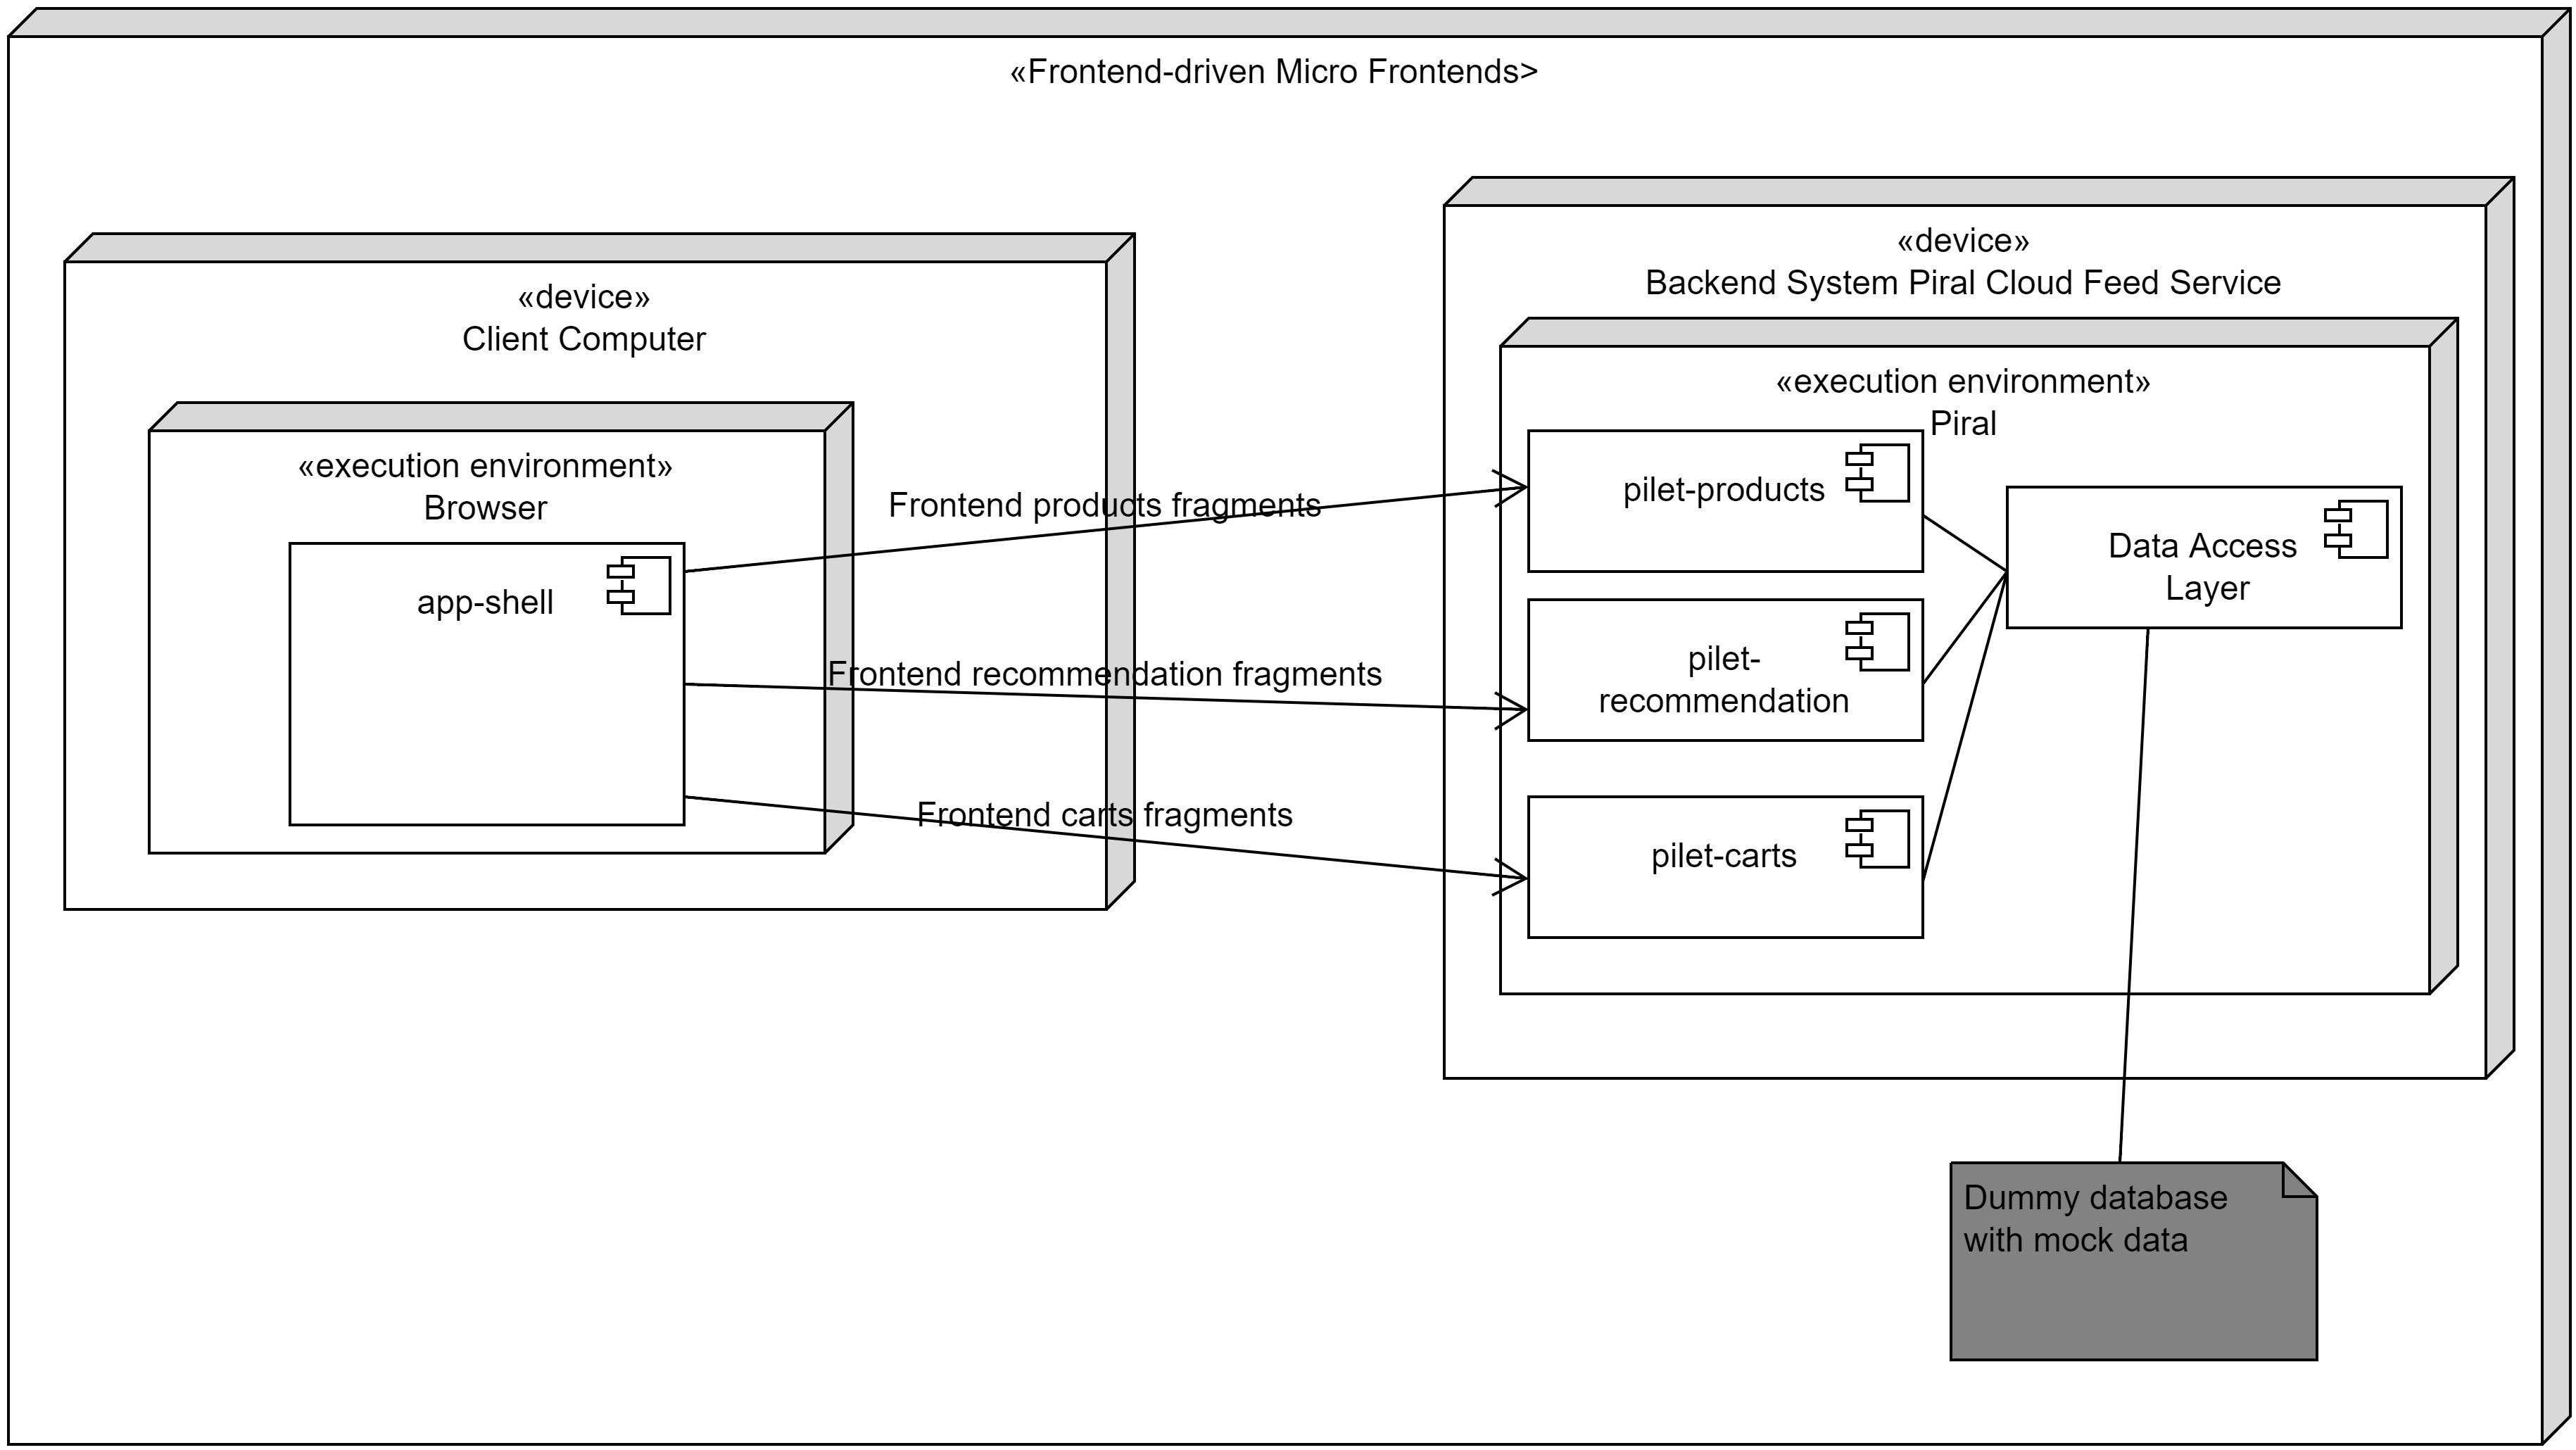
\includegraphics[height=6cm]{piral-architecture-diagram.png}
  \caption{Wild Orchard Store composition}
  \label{fig:piral-architecture-diagram}
\end{figure}
The app-shell is the gateway of the application. App-shell initially and consequently uses, loads and updates different Micro Frontends parts, they are \verb|pilet-products, pilet-recommendation and pilet-carts|.

\subsection{Results}

\begin{table}[h!]
    \captionsetup{justification=centering}
    \caption{Pilets and their locations}
    \label{tab:example_1}
    \centering
    \begin{tabular}{l | cc}
	\toprule
			\textbf{Pilet} & \textbf{Pilet's area}\\
	\midrule
	\textbf app-shell & container and navigation with menu items\\
	\textbf pilet-products              & marked with red border\\
	\textbf pilet-recommendation             & marked with yellow border\\
	\textbf pilet-carts              & marked with blue border\\
	\bottomrule
    \end{tabular}
\end{table}


\begin{figure}[h!]
    \centering
    \captionsetup{justification=centering}
    \subfloat[List of products page]{\includegraphics[width=0.5\hsize]{ui-products-page.png}}
    \hspace*{0.1\hsize}
    \subfloat[Product details page]{\includegraphics[width=0.5\hsize]{ui-product-details2.png}}
    \caption{Pilet-products}
    \label{fig:Pilet-products}
\end{figure}

\begin{figure}[h!]
    \centering
    \captionsetup{justification=centering}
    \subfloat[pilet-recommendation product  ]{\includegraphics[width=0.5\hsize]{ui-product-details3.png}}
    \hspace*{0.1\hsize}
    \subfloat[pilet-carts cart page ]{\includegraphics[width=0.5\hsize]{ui-product-details4.png}}
    \caption{Pilet-recommendation and pilet-carts}
    \label{fig:ui-product-details-repo}
\end{figure}

\begin{figure}[h!]
    \centering
    \captionsetup{justification=centering}
    \subfloat[Starting point]{\includegraphics[width=0.3\hsize]{cj-first-1.png}}
    % \hspace*{0.1\hsize}
    \subfloat[Navigate to new category]{\includegraphics[width=0.3\hsize]{cj-first-2.png}}
    \subfloat[Navigate to another new category]{\includegraphics[width=0.3\hsize]{cj-first-3.png}}
    \caption{Customer Journey of the first use case}
    \label{Customer Journey of 1. Use Case}
\end{figure}

\begin{figure}[h!]
    \centering
    \captionsetup{justification=centering}
    \subfloat[Starting point]{\includegraphics[width=0.3\hsize]{cj-second-1.png}}
    % \hspace*{0.1\hsize}
    \subfloat[Navigate to new item in related products section]{\includegraphics[width=0.3\hsize]{cj-second-2.png}}
    \subfloat[Navigate to another new item in related products section]{\includegraphics[width=0.3\hsize]{cj-second-3.png}}
    \caption{Customer Journey of the second use case (related products section comes from pilet-recommendation, other categories section comes from pilet-products)}
    \label{Customer Journey of 2. Use Case}
\end{figure}

\begin{figure}[h!]
    \centering
    \captionsetup{justification=centering}
    \subfloat[Starting point]{\includegraphics[width=0.4\hsize]{cj-third-1.png}}
    % \hspace*{0.1\hsize}
    \subfloat[Purchase a product]{\includegraphics[width=0.4\hsize]{cj-third-2.png}}
    \caption{Customer Journey of the third use case}
    \label{Customer Journey of 3. Use Case}
\end{figure}

\begin{figure}[h!]
    \centering
    \captionsetup{justification=centering}
    \subfloat[Purchase another product]{\includegraphics[width=0.4\hsize]{cj-third-3.png}}
    % \hspace*{0.1\hsize}
    \subfloat[Navigate to cart page]{\includegraphics[width=0.4\hsize]{cj-third-4.png}}
    \caption{Customer Journey of the third use case (cont)}
    \label{Customer Journey of 3. Use Case}
\end{figure}

%%%%%%%%%%%%%%%%%%%%%%%%%%%%%%%%%%%%%%%%%%%%%%%%%%%%%%%%%%%%%%%%%%%%%%%%%%%%%%%
%% Chapter 5
\chapter{Micro Frontends Technical Implementation} \label{Micro Frontends Implementations}
\textit{This chapter examines Micro Frontends implementations and the results of the study in greater detail with code snippets and practical examples.}
\section{Micro Frontends Integration} 
\subsection{Link and iframe}
A simple and intuitive strategy of implementing Micro Frontends is page-to-page transition via link and composition of fragments using iframe \cite{iframe}.
\\ \\
As for link transition, firstly, the single coupling between teams is the knowledge of other teams’ URL pattern. For instance, a team need only know the exact URL path to a Micro Frontend and hard code it to its web page to make the integration work via a simple click from client. Secondly, link transition meets the expectation of high robustness and low coupling. For instance, if a Micro Frontend goes down, other parts in the whole application still works. In other words, the web application shares nothing. A Micro Frontend has everything it needs to fulfill its task regardless of technical frameworks, programming languages and deployment strategy other teams use or any error they cause.
\\ \\
However, developers cannot embed a Micro Frontend into another, and more sophisticated integration techniques cannot be achieved using links. 
\\ \\
As for iframe transition, it is possible to place one Micro Frontend inside another, yet still preserving loose coupling and robustness properties. Firstly, iframes provides strong technical isolation. For instance, styles in one iframes cannot leak into other components, and script execution is regulated as they include crucial security features to encapsulate the different Micro Frontends.
\\ \\
However, iframe integration is a document-in-document or websites-in-websites approach while direct assembling of HTML fragments is desired in most cases, which requires a Micro Frontend to provide or expose snippet of HTML or valid Web Components later translated into DOM elements within the final DOM context. Iframe also has some major        disadvantages. Firstly, the layout of an iframe’s content is fix and determined in advance. For example, the current host document needs to know the exact height of the including iframe’s content from a remote Micro Frontend. Moreover, responsive design is hard to achieve. In this case, the child iframe’s content has no way to responsively adjust height or width as its dimension is defined by the parent document. Teams end up with a more complicated technical agreements of not only the URLs but also CSS properties. Secondly, iframe is resource-intensive and leads to poor performance for the browser. The browser generates a new context with computing resource such as RAM and CPU for every iframe. Thirdly, iframe is bad for accessibility and search engines.

\begin{figure}[h!]
  \centering
  \captionsetup{justification=centering}
  \includegraphics[height=3cm]{iframe-wireframe.png}
  \caption{Micro Frontends with iframe \cite{Luc21}}
  \label{fig:iframe}
\end{figure}

\subsection{Integration with Piral} \label{Integration with Pira}

\subsubsection{Activating pages, client-side routing}
One of the core features of Piral is routing. The app-shell assumes the task of determining what pages are shown based on the URLs path. Following figure illustrates the standard pattern of routing engines. The app or PiletAPI object is globally installed and used to register and unregister pages of all Micro Frontends. Consequently, URL changes are handled by routing engines. This enables orchestrating multiple pages from one or multiple Micro Frontends in the application.
\begin{figure}[h!]
  \centering
  \captionsetup{justification=centering}
  \includegraphics[height=4cm]{piral-routing.png}
  \caption{A common activator checks all registered micro frontends for their status \cite{Rap20}}
  \label{fig:piral-routing}
\end{figure}

In Piral, each module carries out the page registration step itself via \verb|app.registerPage| and \verb|app.unregisterPage| functions. This takes place within the exposed setup function of each Pilets, often in the root config file \verb|index.tsx|.
\\ \\
Let’s look at an example of the config file \verb|index.tsx| in \verb|pilet-products (pilet-products\src\index.tsx)|.

\begin{lstlisting}[caption={pilet-products index.tsx}]
// ...
import * as React from "react";
import { Redirect } from "react-router-dom";
import { PiletApi } from "app-shell";
import { ProductsPage } from "./components/ProductsPage";
// ..

const ProductDetailsPage = React.lazy(
  // ...
);

export function setup(app: PiletApi) {
  // page resgistrations
  app.registerPage("/landing", ({ history }) => (
    <ProductsPage history={history} />
  ));

// ...
}
\end{lstlisting}

Here the URL path \verb|${host}/landing| is associated with \verb|ProductsPage| React Component. When a webpage with URL path \verb|${host}/landing| is requested, the products page will be shown.
\\ \\
The PiletApi keeps track, orchestrate, and decide which Micro Frontend is currently loaded, should be loaded next and need to be mounted or unmounted.
\subsubsection{Extending, sharing components, or Piral extension}
One of the selling points of Piral is Piral extension, that is using components provided by the Pilets. 
\\ \\
In the sample application, the product details page from \verb|pilet-products| has and use the buy button from \verb|pilet-carts|. 
\\ \\The code looks like this, in \verb|pilet-carts\src\index.tsx|:

\begin{lstlisting}[caption={pilet-carts extension}]
  // ...
  import * as React from "react";
  import { Link } from "react-router-dom";
  import { PiletApi } from "app-shell";
  import { BuyButton } from "./components/BuyButton";
  import { CartPage } from "./components/CartPage";
  
  interface BuyButtonExtension { // ...  }
  
  export function setup(app: PiletApi) {
    // page resgistrations
    app.registerPage("/cart", () => ( // ... ));
    
    app.setData("cart-data", []);
  
    const addToCart = (item) => { // ...  }
  
    app.registerExtension<BuyButtonExtension>("buy-button", ({ params }) => (
      <BuyButton addToCart={addToCart} product={params.product} />
    ));
    // ...
  }
\end{lstlisting}

The code look like this in \verb|pilet-products\src\index.tsx|:

\begin{lstlisting}[caption={pilet-products uses pilet-carts extension}]
  // ...

const ProductDetailsPage = React.lazy(
  () => import("./components/ProductDetailsPage")
);

export function setup(app: PiletApi) {
  // page resgistrations
  app.registerPage("/landing", ({ history }) => ( // ... ));

  app.registerPage("/products/:id?", ({ history, match, piral }) => (
    <ProductDetailsPage
      id={match.params.id || "1"}
      history={history}
      BuyButton={({ product }) => (
        <piral.Extension
          name="buy-button"
          params={{ product }}
          empty={() => (
            <div className="blue-buy" id="buy">
              {" "}
              Buy button from (Micro Frontend) Pilet Carts{" "}
            </div>
          )}
        />
      )}
      Recommendations={({ category }) => ( // ... )}
    />
  ));
  // ...
  }
\end{lstlisting}

Here the \verb|pilet-carts| register an extension name \verb|buy-button| which hosts the \verb|Recommendation| React Component. In \verb|pilet-products|, the \verb|ProductDetailsPage| use the extension via \verb|piral.Extension| API. In this case, the \verb|piral.Extension| with name \verb|buy-button| is passed down to \verb|ProductDetailsPage| in the root config \verb|index.tsx| file. This approach decouples the actual React Component from Piral and improves readability and testability of the code; \verb|empty| property specifies the fallback element if the main application cannot resolve this extension.
\\ \\ 
Moreover, during registration step of a shared component, the name of the Micro Frontend producer need not be mentioned. Alternatively, developers can give the extension an appropriate name. As a result, the application and developers derive the name of an extension by its actual name, instead of directly referencing the name of responsible service.

\begin{figure}[h!]
  \centering
  \captionsetup{justification=centering}
  \includegraphics[height=6cm]{piral-extension-diagram.png}
  \caption{The general flow for components extension \cite{Rap20}}
  \label{fig:extension-diagram}
\end{figure}

\section{Communication Patterns}
In many real-world applications, interaction is the norm. Hence, communication patterns are essential and required in most cases.
\subsection{iFrame Communication}

In the case of iframe, according to Florian Rappl, communication can take place between reusable Frontend pieces by using the \verb|window.postMessage| function since \verb|HTML5|. The first characteristics of \verb|window.postMessage| lies in the way that it only allows strings to be passed. It is obvious that true objects or JavaScript functions cannot be delivered even though strings can be translated into quite complex \verb|JSON-serialized| objects. \cite{Rap20}
\subsubsection{Sending a message}
For example, the following code represents the code for Micro Frontend products, the iframe sends a message data to the target origin \verb|http://localhost:1234/mfe-products|
\begin{lstlisting}[caption={Iframe script of Micro Frontend products}]
<iframe src="http://localhost:1234/mfe-products" name="mfe-products">

<script>
  let productsFrame = window.frames.mfe-products;
  productsFrame.postMessage("message", "http://localhost:1234/pilet-products");
</script>
}
\end{lstlisting}
\subsubsection{Receiving a message}
A handler is responsible for listening to new event when \verb|postMessage| is called. The \verb|event| object has \verb|event.data| property to access the transferred data and \verb|origin| property represents the sender, for instance \verb|http://localhost:1234/app-shell|
\begin{lstlisting}[caption={An iframe script can be properly set up for receiving the message in other iframes}]
  <script>
    window.addEventListener('message', function(event) {
      alert(`Received ${event.data} from ${event.origin}`);
    });
  </script>
}
\end{lstlisting}
\subsection{Piral Communication}
\subsubsection{Top-down Communication}
The first use case (\ref{Customer Journey of 1. Use Case}) is governed by \verb|pilet-products|. In the current product details page, users can navigate and click around different categories of chosen tea, that is matcha, green tea leaves or spring tea series. Consequently, relevant sections, that is related products and buy button with price sections, are updated.
\\ \\
For instance, by clicking to the spring tea category, a new spring tea product page is loaded and the product recommendation section from \verb|pilet-recommendation| as well as buy button with price from \verb|pilet-carts| are updated accordingly. In this case, \verb|pilet-products| initialize a request, communicate new changes to and notify \verb|pilet-recommendation| and \verb|pilet-carts|, the two Pilets consumes these events.
\\ \\
The code look like this in \verb|pilet-products\src\components\ProductDetailsPage.tsx|:
\begin{lstlisting}[caption={ProductDetailsPage passes product data directly to extended components}]
import * as React from "react";
import { History } from "history";
import { products } from "../data/products";
import { productsUniqueCategories } from "../data/productsUniqueCategories";

export interface ProductDetailsPageProps {
  id: string;
  history: History;
  BuyButton: React.ComponentType<{
    product: any;
  }>;
  Recommendations: React.ComponentType<{
    category: string;
  }>;
}

const ProductDetailsPage: React.FC<ProductDetailsPageProps> = ({
  id,
  history,
  BuyButton,
  Recommendations,
}) => {
  const [currentDisplayedProduct] = products.filter(
    (product) => id === product.id
  );

  return (
    currentDisplayedProduct && (
      <>
        <div id="webhop-main">
          <h1 id="store">Wild Orchard Store</h1>
          <h2 id="name"> </h2>
          <p id="description">
            // ...
          </p>
          <div id="imageMain">
            // ...
          </div>
          <BuyButton product={currentDisplayedProduct} />
          <div id="options">
            // ...
          </div>
          <Recommendations category={currentDisplayedProduct.category} />
        </div>
      </>
    )
  );
};
\end{lstlisting}

In short, \verb|pilet-products| communicate and deliver requests to \verb|pilet-recommendation| and \verb|pilet-carts|, that is a top-down communication. 

\subsubsection{Top-up Communication} 
For the second use case (\ref{Customer Journey of 2. Use Case}), in the first glance, this situation seems to be identical with the first one. The main difference is that browsing, clicking and navigating inside related products section involves another Micro Frontend, that is \verb|pilet-recommendation|. 

For instance, when a user clicks to the \verb|AYR Red Powder| image, the current page is updated with information of the new product. In particular, there is no smooth and app-like experience like that of single page application rerouting like \verb|react-router-dom|, instead the browser refreshes the page with updated URL path. The reason for this is simple: \verb|pilet-recommendation| is a separate component and can only notify the \verb|pilet-products| to refresh the page for new contents. In fact, \verb|pilet-recommendation| emits an event with the desired product ID, \verb|pilet-products| listens to this event, receives the product ID from \verb|pilet-recommendation| and carries out the actual navigation on its own. In other words, \verb|pilet-recommendation| does not do the navigation itself, instead it delegates the task to \verb|pilet-products|. 
\\ \\
The code look like this in \verb|pilet-products\src\index.tsx|:
\begin{lstlisting}[caption={pilet-products listens to custom event and carries out the navigation}]
  // ...
  // Event from Recommendation pilet
  // Pilet Products carries out the actual navigation
  app.on("recommendation-click-event", (data) => {
    const navigateToNewPage = () => {
      history.push(`/products/${data.id}`);
      window.location.reload();
    };
    return navigateToNewPage();
  });
  // ...
  }
\end{lstlisting}


The code look like this in \verb|pilet-recommendation\src\index.tsx|:
\begin{lstlisting}[caption={pilet-recommendation emits custom event and transmits the product Id}]
import * as React from "react";
import { PiletApi } from "app-shell";
import { Recommendations } from "./components/Recommendations";

interface RecommendationExtension {
  category: string;
}

export function setup(app: PiletApi) {
  const emitEventData = (id) => {
    app.emit("recommendation-click-event", {
      id,
    });
  };

  app.registerExtension<RecommendationExtension>(
    "recommendations",
    ({ params }) => (
      <Recommendations category={params.category} navigate={emitEventData} />
    )
  );
}
\end{lstlisting}

\begin{figure}[h!]
  \centering
  \captionsetup{justification=centering}
  \includegraphics[height=4cm]{piral-event-diagram.png}
  \caption{The standard DOM event interface can be used to exchange events \cite{Rap20}}
  \label{fig:piral-event-diagram}
\end{figure}

This case is a top up communication via events between Micro Frontends, from \verb|pilet-recommendation| upward to \verb|pilet-products|.  

\subsubsection{Sharing data between Pilets}

\begin{figure}[h!]
  \centering
  \captionsetup{justification=centering}
  \includegraphics[height=4cm]{piral-global-context-diagram.png}
  \caption{A central API provides read and write access to shared data \cite{Rap20}}
  \label{fig:piral-global-context-diagram}
\end{figure}

The last use case is cart function (\ref{Customer Journey of 3. Use Case}). Users click to the buy button, the cart navigator on top-right corner is updated accordingly, and cart data can be seen on cart page.
\\ \\ 
The use case essentially involves \verb|pilet-carts|, \verb|app-shel|l, and requires \verb|pilet-products|. When users click buy button, the products data are saved (in memory) and later can be retrieved on cart page. In this case, \verb|pilet-cart|s uses, updates and keep track of the state of cart data. The state of cart data is universally shared and accessed by any Pilet and the app-shell with \verb|setData| and \verb|getData| methods of Pilet API. It then updates the Cart menu item in app-shell every time new data arrives via Piral global state management mechanism. Eagle eye readers may notice that especially in the second use case, the cart data is reset. This is inevitable due to in memory storage and lack of proper and persistent state management. This is acceptable for the purpose of illustration.
\\ \\
The code look like this in \verb|pilet-carts\src\index.tsx|:
\begin{lstlisting}[caption={pilet-carts handles cart data}]
import * as React from "react";
import { Link } from "react-router-dom";
import { PiletApi } from "app-shell";
import { BuyButton } from "./components/BuyButton";
import { CartPage } from "./components/CartPage";

interface BuyButtonExtension {
  product: any;
}

export function setup(app: PiletApi) {
  // page resgistrations

  app.registerPage("/cart", () => ( // ... ));

  app.setData("cart-data", []);

  const addToCart = (item) => {
    var cart = app.getData("cart-data");
    cart.push(item);
    app.setData("cart-data", cart);
    console.log("Cart: ", cart);
  };

  app.registerExtension<BuyButtonExtension>("buy-button", ({ params }) => ( // ...));

  // Cart event
  app.registerMenu("cart-menu", () => { // ...});

  app.on("store-data", ({ name }) => {
    if (name === "cart-data") {
      app.registerMenu("cart-menu", () => (
        <Link to="/cart">Cart - {app.getData("cart-data").length} </Link>
      ));
    }
  });
}

\end{lstlisting}

\section{Lazy Loading}
Instead of downloading all information on initial loading to a web application, a component is loaded at its first use case. Then, lazy loading reduces initial load time, reduces page weight leading to quicker page load time, and conserving bandwidth by avoiding requesting unused data and resources.
\\ \\
The code look like this in \verb|pilet-products\src\index.tsx|:
\begin{lstlisting}[caption={Lazy loading of a React component in pilet-products index.tsx file}]
  // ...
const ProductDetailsPage = React.lazy(
  () => import("./components/ProductDetailsPage")
);

export function setup(app: PiletApi) {
  // page resgistrations
  app.registerPage("/landing", ({ history }) => ( 
    <ProductsPage history={history} />
  ));

  app.registerPage("/products/:id?", ({ history, match, piral }) => (
    <ProductDetailsPage
      id={match.params.id || "1"}
      history={history}
      BuyButton={({ product }) => ( // ... )}
      Recommendations={({ category }) => ( // ... )}
    />
  ));
  // ...
  }
\end{lstlisting}
On initial load, user is navigated to list of all products page. Then, only when moving to product details page does the browser download the code for \verb|ProductDetailsPage| React component. Lazy loading is implemented via \verb|React.lazy()|\cite{ReactLazy} in this case.

\section{Dependencies Management}
Sharing dependencies is an appropriate setting in Micro Frontends. In practice, developers can take either way of sharing dependencies: sharing no dependencies as it is the case in Microservices or sharing all inter-team dependencies. For getting best of both worlds, however, developers have to decide which dependencies to share.
\\ \\
Firstly, in the beginning, it is not necessary for every Micro Frontend to share all dependencies, instead they should always share nothing. It is reasonable that so doing will make it easy for developers to familiarize themselves with an unfamiliar coding environment, avoid configuration constraints, potential bugs and inessential complexities. However, including every required dependency in each Micro Frontend in this manner makes the whole application slow and bloated, finally worsening its performance. Then, what really matters is how developers should decide which dependencies to share. In Micro Frontends world, this decision is justified on the basis of performance-based assessment and evaluation. According to Florian Rappl \cite{Rap20}, some criteria are:
\begin{quote}
    \textit{
\begin{itemize}
    \item They should be of a significant size (from at least 15 KB to 30 KB; even more
appropriate is 100 KB)
    \item They should be used by at least two micro frontends.
    \item They should not have multiple commonly used versions with breaking changes.
    \item They should play an important role in rendering components
    \item They should be technical, not domain specific
\end{itemize}
}
\end{quote}

One worth mentioning point is that increasing demand for domain specific dependencies often indicate domain decomposition and architectural boundaries have developed faults or undergone beforehand some incorrect steps for instance during requirement engineering process. In this case, developers should fall back to previous software engineering stages and improve them before eventually adding more shared dependencies. Once a shared dependency is included, it is coupled to the system and generally impossible to reverse.
\\ \\ 
Secondly, how should this functionality be realized? 
\\ \\ 
\textbf{
Sharing dependencies in Webpack Module Federation
}
\\ \\ 
Webpack Module Federation offers Micro Frontends a way to exchange dependencies freely:
\begin{lstlisting}[language=Python]
// ...
const ModuleFederationPlugin = require("webpack/lib/container/ModuleFederationPlugin");
// ...

const devConfig = {
  // ...
  plugins: [
    new ModuleFederationPlugin({
      name: "app-shell",
      // ...
      // sharing dependencies
      shared: packageJson.dependencies,
    }),
  ],
};

// ...
\end{lstlisting}
A selling point of Module Federation is the ability to add additional constraints such as dependencies versions. This allows finer control at selecting only dependencies with match versions.
\\ \\
\textbf{
Sharing dependencies in Piral
}
\\ \\ 
Let’s say we have three Micro Frontends \verb|pilet-products|, \verb|pilet-recommendation| and \verb|pilet-carts|. All of them use the same framework that is React. Moreover, they can use additional libraries such as React Router DOM. In this case developers need a way to allow they use one single dependency of React.
\\ \\ 
In Piral, sharing dependencies is straight forward. The easiest way to share dependencies from the app shell is to declare them in the externals section of the \verb|package.json|. For instance, if we want to share vue dependency we can extend \verb|pilet.external| in the app shell's \verb|package.json|:

\begin{lstlisting}{language=Python}
// ...
"pilets": {
    "files": [],
    "externals": [
      "vue"
    ],
    // ...
}
// ...
\end{lstlisting}
One worth mentioning point is that the following dependencies are shared and default dependencies used in Piral, hence always added:
\begin{itemize}
    \item react
    \item react-dom
    \item react-router
    \item react-router-dom
    \item history
    \item tslib
    \item path-to-regexp
    \item @libre/atom
    \item @dbeining/react-atom
    
\end{itemize}
Any other dependency needs to be added to the externals list.
Here is an example of sharing dependencies of pilet-products where they are listed in \verb|peerDependencies| property.
\begin{quote}
The peerDependencies represent the list of shared dependency libraries, i.e., dependencies treated as external, which are shared by the application shell. The peerModules repesent the list of shared dependency modules, i.e., modules treated as external, which are shared by the application shell. (\url{https://docs.piral.io/reference/documentation/metadata})

\end{quote}
\begin{lstlisting}{language=Python}
// ...
"peerDependencies": {
    "@dbeining/react-atom": "*",
    "@libre/atom": "*",
    "app-shell": "*",
    "history": "*",
    "path-to-regexp": "*",
    "react": "*",
    "react-dom": "*",
    "react-router": "*",
    "react-router-dom": "*",
    "tslib": "*"
  },
// ...
\end{lstlisting}

A real-world sharing dependencies scenario from the sample application:
\\ \\
\begin{figure}[h!]
    \centering
    \captionsetup{justification=centering}
    \includegraphics[height=6cm]{piral-dependencies.png}
    \caption{Dependencies in Piral. All three Pilets use one single react package}
    \label{fig:4}
\end{figure}

The downside of this pattern is increased coordination and overall complexity. In the end, developers presumably get the best of both worlds: more flexibility and better performance. 
\section{Knowledge sharing }
In practice, it is the case that communicating changes such as API changes and event production will be of concern for scaling development. 
\\ \\
Firstly, agreements, conventions and contracts need to be formed among teams. For instance, if a Micro Frontend expose an event with a certain name, this information needs to be shared to all consumers. In the case of event name changes, the responsible team must do the job of keeping consuming teams informed about the changes.
\begin{figure}[h!]
    \centering
    \captionsetup{justification=centering}
    \includegraphics[height=6cm]{knowledge-sharing-event.png}
    \caption{Change of event's name \cite{Rap20}}
    \label{fig:5}
\end{figure}
Secondly, autonomy is good, productivity is better and communication factor plays an important role. Adopting shared load test [Ref] scenarios or picking a common error-logging infrastructure without reinventing the wheels should always be taken as a long-lasting productive method concerning high-quality, focused idea development, effective time management, and possible risk management. Transparent protocol for information exchange should be available in most cases.
\\ \\
Thirdly, ensuring visual consistency across Micro Frontends is vital for the final product. A style guide and design system including user interface like form, navigation, menu item, input field, button, icon or typography can be made public, accessible for every party, serve as a guideline and reference for developers.

\section{Cross-framework Components}
Piral is based on React and utilizes plugin architecture to allow components from other frameworks to be integrated. For example, in the context of one Pilet, to use \verb|vue| components, developers need to install Piral plugin for \verb|vue|: \verb|piral-vue|.

\begin{lstlisting}[caption={Setup to integrate Vue components in a Pilet}]
# Add the plugin to your Piral instance by running:
npm i piral-vue
# Install vue
npm i vue

\end{lstlisting}
The following function for cross-frameworks integration is then added to the Pilet API: \verb|fromVue()|
% \begin{item}
%     \item \verb|fromVue()|: \begin{quote}
%         Transforms a standard Vue@2 component into a component that can be used in Piral, essentially wrapping it with a reference to the corresponding converter.
%     \end{quote}
% \end{item}\
\\ \\
Use a \verb|vue| component in a Pilet:

\begin{lstlisting}[caption={Piral docs Vue plugin \url{https://docs.piral.io/plugins/piral-vue/overview}}]
import { PiletApi } from "app-shell";
import { fromVue } from 'piral-vue/convert';
import VuePage from "./Page.vue";
import BuyButton from "./BuyButton.vue";

interface BuyButtonExtension {
  item: Object
}

export function setup(app: PiletApi) {

  const addToCart = (item) => {
    // ...
  }
  
  app.registerPage('/sample', app.fromVue(VuePage));
  
  app.registerExtension<BuyButtonExtension>(
    'buy-button', 
    app.fromVue(BuyButton, { addToCart: addToCart}})
  )
}

\end{lstlisting}

% A Vue extension can be used by following code:

% \begin{lstlisting}[caption={Code snippet from Piral docs}]

% <extension-component name="name-of-extension"></extension-component>

% \end{lstlisting}

Naturally, framework's specific modules and tools such as \verb|vue vue-loader vue-template-compiler| need to be installed via \verb|npm|. The final dependencies can be like so:
\begin{lstlisting}[caption={Vue realted dependencies in a Pilet}]
// ...
"dependencies": {
    "@vue/component-compiler-utils": "^3.3.0",
    "piral-vue": "^0.14.24",
    "vue": "^2.0.2",
    "vue-loader": "^17.0.0",
    "vue-template-compiler": "^2.0.2"
  }
// ...

\end{lstlisting}

Incompatible framework's version of components for instance \verb|vue@\^2.0.0| and \verb|vue@\^3.0.0| plays no role in this case, as long as the setup is properly handled.

% \section{Exchange of Cross-framework Components}
% \section{Consistency}
\section{Reliability}
According to James Lewis, as a consequence of utilizing distributed systems, applications need to handle failure of services properly if one of them is unavailable due to some reason, introducing an additional layer of complexity, yet making the software in one way or another more resilient to failure. \cite{Lew14}
\\ \\
Established approach such as \textit{“setting small timeouts, implementing retries for implementing retries for high-priority requests and detecting a connection loss so as to handle it gracefully”} \cite{Rap20} should be applied. Even though, developers need to handle exception and error properly. In this case, error boundary can be used. Prominent example is React Error Boundaries \cite{ReactErrorBundaries} and Piral fallback mechanism. Furthermore, cancellation of a Micro Frontend service will support testing, help ensure scaling development and loose coupling. The next section gives some insights into this topic.

\section{Cancellation of a Micro Frontend Service}
Regarding the reliability of Piral apps, let's try disable the two Pilets \verb|pilet-carts| and \verb|pilet-recommendation|:
\begin{figure}[h!]
  \centering
  \captionsetup{justification=centering}
  \includegraphics[height=6cm]{piral-feed-service-deactivated.png}
  \caption{Deactivate the Pilets}
  \label{fig:piral-feed-service-deactivated}
\end{figure}

Piral provides fallback mechanism for an extension with property \verb|empty| out of the box, in \verb|pilet-products\src\index.tsx|, the code looks like this:

\begin{lstlisting}[caption={pilet-products index.tsx}]
  export function setup(app: PiletApi) {
  // ...

  app.registerPage("/products/:id?", ({ history, match, piral }) => (
    <ProductDetailsPage
      id={match.params.id || "1"}
      history={history}
      BuyButton={({ product }) => (
        <piral.Extension
          name="buy-button"
          params={{ product }}
          empty={() => (
            <div className="blue-buy" id="buy">
              {" "}
              Buy button from (Micro Frontend) Pilet Carts{" "}
            </div>
          )}
        />
      )}
      Recommendations={({ category }) => (
        <piral.Extension
          name="recommendations"
          params={{ category }}
          empty={() => (
            <div className="green-recos" id="reco">
              {" "}
              Recommendation products from (Micro Frontend) Pilet Recommendation{" "}
            </div>
          )}
        />
      )}
    />
  ));

  // ...
}
\end{lstlisting}

Failure in one Micro Frontend can be properly handled to avoid affecting other parts of the application. Moreover, in light of section \ref{IsolatedFeatures}, feature extension and improvement takes place without the consequence
of editing the same UI simultaneously. The end-result:

\begin{figure}[h!]
  \centering
  \captionsetup{justification=centering}
  \includegraphics[height=6cm]{wireframe.png}
  \caption{pilet-carts and pilet-recommendation are unavailable}
  \label{fig:wireframe1}
\end{figure}

\section{Request optimizations for Performance}
Micro Frontends leading to modularization calls developers’ attention to growing API requests as in place of a monolith, a much more fragmented system, both server- and client-side, comes into being. The sum total of HTTP requests increase as a consequence. In this case, if many modules query the same data, a best practice to mitigate this effect is micro-caching for API requests. \cite{Rap20}

\section{Performance of Multiple Frameworks Micro Frontends}
According to Luca, using multiple frameworks like React, Angular, Vue, or Svelte in Micro Frontends leads to larger payload size, potential dependency clashes and much overhead. For instance, assume having multiple versions of React and a version of Angular in the same view, the browser needs to download several versions of React and one version of Angular, resulting large download size for client users and potential conflicts of global variables among different libraries. However, there are cases where this approach make sense, for example, in dealing with old or outdated framework's version and migrating a legacy application to a new one. There are several solutions for the multi-framework approach. \cite{Luc21}
\begin{quote}
    \textit{"Iframes create a
sandbox so that what loads inside one iframe doesn’t clash with another
iframe. Module Federa   tion allows you to share libraries and provides a
mechanism for avoiding clashing dependencies. Import maps allow us to
define scopes for every dependency so we can define different versions of
the same libraries to different scopes. And web components can “hide”
behind the shadow DOM the frameworks need for a micro-frontend."} \cite{Luc21}
\end{quote}

\section{CSS Scoping}
Micro Frontends with independent teams make it possible for CSS classes to have duplicate names, leading to some weird behavior on the overall layout. One simple yet resilient and widely adopted practice is prefixing the Micro Frontends name to CSS class. For example:
\begin{lstlisting}[caption={pilet-products CSS prefixing \cite{Luc21}}]
  .avatar {}
  .avatar__image {}
  .avatar__image--active {}
  .avatar__image--inactive {}
  
  // to
  .products_avatar {}
  .products_avatar__image {}
  .products_avatar__image--active {}
  .products_avatar__image--inactive {}
}
\end{lstlisting}

\section{Debugging}
\section{Failure Handling}
% \section{Responsive Design in Micro Frontends}

% \section{Security}
% [...]
\chapter{Evaluation of Piral Sample Application} \label{Evaluation of Piral Sample Application}
\textit{This chapter evaluates the sample application with respect to development and testing as results of the study.}
\section{Developer Experience}
\subsection{Setup}
In the context of section \ref{fig:piral-setup}:
\begin{lstlisting}[caption={Complete setup with Piral}]
# Install the Piral CLI
npm i piral-cli -g

# Scaffold an application shell
piral new --target app-shell

# Create an npm package for the app shell, later referenced by the pilets
npx piral build

# Scaffold a new pilet with with the path to the tarball of the app-shell
pilet new ./app-shell/dist/emulator/app-shell-1.0.0.tgz --target pilet-products
pilet new ./app-shell/dist/emulator/app-shell-1.0.0.tgz --target pilet-recommendation
pilet new ./app-shell/dist/emulator/app-shell-1.0.0.tgz --target pilet-carts

# Start the Piral instance in debug mode
npx piral debug
\end{lstlisting}
By default, the app-shell is started on http://localhost:1234 with the content of the pilets. As we can see, in Piral, scaffolding process is provided out of the box.

\subsection{Micro Frontends Development Cycle}
For every Pilet, a developer can more or less make changes on a unit independently without causing unnecessary and unwanted effects on other parts of the system. 

\begin{lstlisting}[caption={Publishing Pilets \url{https://docs.piral.io/guidelines/tutorials/03-publishing-pilets}}]
# the url of Piral cloud feed service
const feedUrl = 'https://feed.piral.cloud/api/v1/pilet/my-tutorial-feed';

# debug a Pilet locally
pilet debug

# publish a Pilet to the feed service
npx pilet publish --fresh --url https://feed.piral.cloud/api/v1/pilet/my-tutorial-feed --api-key <your-api-key>
\end{lstlisting}

In principle, every Pilet can be developed, built and published, only with some coordination with the app-shell.
\section{Testing}

Unit testing was carried out using \verb|piral-jest-utils| (\url{https://github.com/smapiot/piral/tree/develop/src/utilities/piral-jest-utils}) dependency which provides React Typescript unit test with Jest \cite{Jest} functionality.

\begin{lstlisting}[caption={piral-jest-utils installation with recommended versions}]
  npm install --save-dev piral-jest-utils@^0.14.24 jest@^26.0.0 ts-jest@^26.0.0 @types/jest@^26.0.24
\end{lstlisting}

Due to incompatibility issues with the latest version of React 17 in the time of writing and the fact that both \verb|Jest| and \verb|piral-jest-utils| are a bit outdated, readers might need to install the dependencies in a forceful manner. Following code worked fine with the sample application and should have no major trouble in other settings.

\begin{lstlisting}[caption={piral-jest-utils installation in force mode}]
  npm install --save-dev piral-jest-utils@^0.14.24 jest@^26.0.0 ts-jest@^26.0.0 @types/jest@^26.0.24 --force 
\end{lstlisting}

In \verb|pilet-products\src\test\ProductDetailsPage.test.tsx|, for an example of \verb|pilet-products| unit testing, the code look like this:

\begin{lstlisting}[caption={ProductDetailsPage.test.tsx}]
  import * as React from "react";
import { History } from "history";
import ProductDetailsPage from "../components/ProductDetailsPage";
import { shallow, render } from "enzyme";

const TestDummyComponent = () => <div />;

describe("ProductDetailsPage", () => {
  it("renders", () => {
    render(
      <ProductDetailsPage
        id={"1"}
        history={{} as any as History}
        BuyButton={TestDummyComponent}
        Recommendations={TestDummyComponent}
      />
    );
  });

  it("calls history push", () => {
    const push = jest.fn();
    const wrapper = shallow(
      <ProductDetailsPage
        id={"1"}
        history={{ push } as any as History}
        BuyButton={TestDummyComponent}
        Recommendations={TestDummyComponent}
      />
    );

    wrapper.find("button").first().simulate("click");
    expect(push).toHaveBeenCalled();
  });
});
\end{lstlisting}

The above tests verifies correct rendering of the main component \verb|ProductDetailsPage| and mocks button click for navigation within the pilet. By running the test with commen \verb|npm test| inside the root location \verb|pilet-products\package.json| like so:

\begin{lstlisting}[caption={pilet-products package.json file}]
 // ...
"scripts": {
    "start": "pilet debug",
    "build": "pilet build",
    "upgrade": "pilet upgrade",
    "test": "jest --passWithNoTests"
  },
   // ...
\end{lstlisting}

The test results look like this:

\begin{lstlisting}[caption={pilet-products unit testing results}]
> pilet-products@1.0.64 test
> jest --passWithNoTests    

 PASS  src/test/ProductsPage.test.tsx
  ProductsPage
    √ renders (18 ms)

 PASS  src/test/ProductDetailsPage.test.tsx
  ProductDetailsPage
    √ renders (10 ms)
    √ calls history push (8 ms)

-------------------------------|---------|----------|---------|---------|-------------------
File                           | % Stmts | % Branch | % Funcs | % Lines | Uncovered Line #s
-------------------------------|---------|----------|---------|---------|-------------------
All files                      |      95 |       75 |    87.5 |   94.73 |
 components                    |   94.44 |       75 |    87.5 |   94.11 |
  ProductDetailsPage.tsx       |     100 |       75 |     100 |     100 | 58
  ProductsPage.tsx             |   85.71 |      100 |   66.66 |   83.33 | 38
 data                          |     100 |      100 |     100 |     100 |
  products.tsx                 |     100 |      100 |     100 |     100 |
  productsUniqueCategories.tsx |     100 |      100 |     100 |     100 |
-------------------------------|---------|----------|---------|---------|-------------------
Test Suites: 2 passed, 2 total
Tests:       3 passed, 3 total
Snapshots:   0 total
Time:        5.786 s
Ran all test suites.

\end{lstlisting}

Finally, we have a running sample application verified by proper unit testing.
% \section{Performance }
% Time to first byte, bundle size, \url{https://web.dev/vitals/}


%% Chapter 11

\chapter{Summary and Conclusion}
\section{Summary}
The study is structured as follows. Chapter 2 begins the study by presenting the context of this work. Chapter 3 provides a theoretical background of software architecture, centers around Microservices major principles and characteristics. Chapter 4, 5 and 6 discuss the establishment, characteristics, common problems, advantages and disadvantages of Micro Frontends and popular application architectures. Chapter 7 and 8 are meant for examining client-side composition Micro Frontends theoretically and practically with two prototypes, one with Web Components, one with Piral. Chapter 9 provides a thorough walk-through of the results of the study including sample applications, applications use cases and workflows, detailed images of the final results, and lists out the Micro Frontends components which shape the final app. Chapter 10 dives deep into implementations' details and discuss technical implications of the prototypes and Micro Frontends in general, investigate them in detail, give insights into actual realization of the architecture, and discuss their issues. Chapter 11 highlights the selling points of Piral regarding development process, analyzes and evaluates the sample applications empirically with unit testing. Chapter 12 draws the conclusions.
\section{Conclusion}
The study presents major ideas, characteristics of Micro Frontends, motivations leading to the architecture adoption, and the results of client-side composition Miro Frontends implementation with prototypes using Web Components and Piral. The main findings of the study confirm that Micro Frontends make it possible to bring many benefits of Microservices on the Frontend side, especially scaling development processes, mean much for developers in dealing with typical problems of monolithic systems and attract interest in Micro Frontends as an alternative organizational approach. This work should also help practitioners and researchers familiarize themselves with the possibly unfamiliar concept of Micro Frontend, clarify the architecture most common problems and how to solve them as well as distinguish the pros and cons in different cases. Focus of the study, the approach of client-side composition provides a functional, dynamic and powerful application with clear techniques and sheds light on the architecture's impact on development, production and operation processes.
\\ \\
On the other hand, Micro Frontends do come with significant costs. Potential performance issues, universal design systems, communication overheads, cross-cutting concerns and overall complexity need to be thoroughly investigated and require careful planning, high level of expertise to implement. Moreover, as new tools continuously emerge, no single technology has dominated the market of Micro Frontends

% Further research is needed to carefully
% investigate this new hype, 

% \begin{quote}

% So, software developers often choose to adopt one architecture over another based on their experience in previous projects or based on the perceived benefits of the new architecture. Therefore, it is important to study why Micro-Frontends have been adopted, to understand the current motivations behind their adoption, and to investigate whether specific issues are believed to require more improvement than others. To elicit these motivations, we conducted an empirical study in the form of a Multivocal Literature Review (MLR)

% To the best of our knowledge, only a limited number of studies have investigated Micro-Frontends [7,8]. This work will help companies to understand how Micro-Frontends can be beneficial for their needs, and if motivations, issues and benefits that other companies experienced match their expectancy. Moreover, this work can help researchers to understand the new trend, while at the same time opening up new avenues for future research on web front-ends.
% [...
%  Dynamic behavior of applications
% Developer experience with Piral
% Provide proof of concept, prototypes empirically 
% Target of the study
% Web components using web standards, framework agnostic approach...]
% \end{quote}



%%%%%%%%%%%%%%%%%%%%%%%%%%%%%%%%%%%%%%%%%%%%%%%%%%%%%%%%%%%%%%%%%%%%%%%%%%%%%%%
%% Bibliography

\clearpage
\addcontentsline{toc}{chapter}{Bibliography}
\bibliographystyle{IEEEtran}
\bibliography{references}
%% Harvard style citations with alphebetically sorted bibliography
%%     Must be used with \usepackage[sort&compress]{natbib} in the document preamble
%\bibliographystyle{kluwer}

%% Vancouver style citations with bibliography sorted by appearance of reference
%%     Must be used with \usepackage[sort&compress,numbers]{natbib} in the document preamble

% \bibliographystyle{IEEEtran}  % a common used one in engineering 
% \bibliographystyle{unsrtnat}

% \bibliography{literatur}

%%%%%%%%%%%%%%%%%%%%%%%%%%%%%%%%%%%%%%%%%%%%%%%%%%%%%%%%%%%%%%%%%%%%%%%%%%%%%%%
%% Appendix

% \clearpage
\addcontentsline{toc}{chapter}{Appendix}

\begin{appendix}
\chapter{Source Codes Structure}
Following illustrations present the structure of the sample application. Universally, main contents of a Pilet are \verb|components| directory contains the UI elements, \verb|test| directory contains the testing files, a \verb|tarball| or \verb|tgz| extension file is the production ready version of the Pilet for publishing to feed service, \verb|dist| directory is the release bundle, \verb|node_modules| is dependencies file managed by \verb|npm|, \verb|coverage| directory and \verb|jest.config.js| file are used by \verb|Jest| for testing, finally \verb|data| and \verb|assets| directories contain mock data for the sample application.

\begin{figure}[h!]
  \centering
  \captionsetup{justification=centering}
  \includegraphics[height=2.5cm]{piral-app-monorepository-structure.png}
  \caption{The monorepository consists of four repositories}
  \label{fig:1}
\end{figure}

\begin{figure}[h!]
    \centering
    \captionsetup{justification=centering}
    \subfloat[pilet-products repository]{\includegraphics[width=0.3\hsize]{pilet-products-directory-structure.png}}
    \hspace*{0.1\hsize}
    \subfloat[pilet-recommendation repository]{\includegraphics[width=0.3\hsize]{pilet-recommendation-directory-structure.png}}
    \hspace*{0.1\hsize}
    \subfloat[pilet-carts repository]{\includegraphics[width=0.3\hsize]{pilet-carts-directory-structure.png}}
    \caption{Repository structure of three Pilets}
    \label{fig:monorepositroy}
\end{figure}

\chapter{Testing Results}  %% Use if needed

Following figures present the testing results of the sample application.

\begin{figure}[h!]
    \centering
    \captionsetup{justification=centering}
    \caption{pilet-products testing results}
    {\includegraphics[width=12cm]{test-pilet-products.png}}
\end{figure}

\begin{figure}[h!]
    \centering
    \captionsetup{justification=centering}
    \caption{pilet-recommendation testing results}{\includegraphics[width=12cm]{test-pilet-recommendation.png}}
\end{figure}

\begin{figure}[h!]
    \centering
    \captionsetup{justification=centering}
    \caption{pilet-carts testing results}{\includegraphics[width=12cm]{test-pilet-carts.png}}
\end{figure}


\end{appendix}

%%%%%%%%%%%%%%%%%%%%%%%%%%%%%%%%%%%%%%%%%%%%%%%%%%%%%%%%%%%%%%%%%%%%%%%%%%%%%%%
%% Close document
\end{document}
%%%%%%%%%%%%%%%%%%%%%%%%%%%%%%%%%%%%%%%%%%%%%%%%%%%%%%%%%%%%%%%%%%%%%%%%%%%%%%%
